\documentclass[12pt,a4paper]{article}

% ===== PACKAGES =====
\usepackage[utf8]{inputenc}
\usepackage[vietnamese]{babel}
\usepackage{amsmath,amsfonts,amssymb}
\usepackage{graphicx}
\usepackage{geometry}
\usepackage{fancyhdr}
\usepackage{hyperref}
\usepackage{listings}
\usepackage{xcolor}
\usepackage{booktabs}
\usepackage{longtable}
\usepackage{array}
\usepackage{float}
\usepackage{caption}
\usepackage{subcaption}
\usepackage{enumitem}
\usepackage{tikz}
\usepackage{multirow}
\usepackage{tocloft}
\usepackage{titlesec}

% ===== PAGE SETUP =====
\geometry{
    top=2.5cm,
    bottom=2.5cm,
    left=3cm,
    right=2cm
}

% ===== COLORS =====
\definecolor{codegreen}{rgb}{0,0.6,0}
\definecolor{codegray}{rgb}{0.5,0.5,0.5}
\definecolor{codepurple}{rgb}{0.58,0,0.82}
\definecolor{backcolour}{rgb}{0.95,0.95,0.92}
\definecolor{myblue}{RGB}{0,102,204}

% ===== CODE LISTING STYLE =====
\lstdefinestyle{mystyle}{
    backgroundcolor=\color{backcolour},   
    commentstyle=\color{codegreen},
    keywordstyle=\color{magenta},
    numberstyle=\tiny\color{codegray},
    stringstyle=\color{codepurple},
    basicstyle=\ttfamily\footnotesize,
    breakatwhitespace=false,         
    breaklines=true,                 
    captionpos=b,                    
    keepspaces=true,                 
    numbers=left,                    
    numbersep=5pt,                  
    showspaces=false,                
    showstringspaces=false,
    showtabs=false,                  
    tabsize=2,
    frame=single
}
\lstset{style=mystyle}

% ===== CUSTOM BOX =====
\usepackage{tcolorbox}
\tcbuselibrary{skins,breakable}
\newtcolorbox{definitionbox}[1][]{
    colback=blue!5,
    colframe=myblue,
    fonttitle=\bfseries,
    title=#1,
    breakable
}

% ===== HEADER/FOOTER =====
\pagestyle{fancy}
\fancyhf{}
\fancyhead[L]{\leftmark}
\fancyhead[R]{Đồ án cuối kỳ - Python cho KHĐL}
\fancyfoot[C]{\thepage}
\renewcommand{\headrulewidth}{0.4pt}
\renewcommand{\footrulewidth}{0.4pt}

% ===== HYPERLINK SETUP =====
\hypersetup{
    colorlinks=true,
    linkcolor=myblue,
    filecolor=magenta,      
    urlcolor=cyan,
    pdftitle={Đồ án Dự đoán Giá Taxi},
    pdfauthor={Sinh viên K23},
}

% ===== TITLE FORMATTING =====
\titleformat{\section}
  {\normalfont\Large\bfseries\color{myblue}}{\thesection}{1em}{}
\titleformat{\subsection}
  {\normalfont\large\bfseries}{\thesubsection}{1em}{}
\titleformat{\subsubsection}
  {\normalfont\normalsize\bfseries}{\thesubsubsection}{1em}{}

\begin{document}

% ===== TRANG BÌA =====
\begin{titlepage}
    \centering
    \vspace*{1cm}
    
    {\Large\textbf{TRƯỜNG ĐẠI HỌC ...}}\\[0.3cm]
    {\large\textbf{KHOA CÔNG NGHỆ THÔNG TIN}}\\[0.5cm]
    
    \vspace{1cm}
    \rule{\linewidth}{0.5mm}\\[0.4cm]
    {\Huge\bfseries ĐỒ ÁN CUỐI KỲ}\\[0.2cm]
    {\Large\textbf{Môn: Python cho Khoa học Dữ liệu}}\\[0.2cm]
    \rule{\linewidth}{0.5mm}\\[1cm]
    
    {\LARGE\bfseries DỰ ĐOÁN GIÁ CƯỚC TAXI}\\[0.3cm]
    {\Large Sử dụng Machine Learning Pipeline}\\[2cm]
    
    \begin{minipage}{0.5\textwidth}
        \begin{flushleft}\large
            \textbf{Sinh viên thực hiện:}\\
            1. [Họ tên SV 1] - [MSSV]\\
            2. [Họ tên SV 2] - [MSSV]\\
            3. [Họ tên SV 3] - [MSSV]
        \end{flushleft}
    \end{minipage}
    ~
    \begin{minipage}{0.4\textwidth}
        \begin{flushright}\large
            \textbf{Giảng viên hướng dẫn:}\\
            [Tên GV]
        \end{flushright}
    \end{minipage}\\[3cm]
    
    \vfill
    {\large Khóa: K23}\\
    {\large Năm học: 2024 - 2025}
    
\end{titlepage}

% ===== MỤC LỤC =====
\tableofcontents
\newpage

% ===== DANH MỤC HÌNH ẢNH =====
\listoffigures
\newpage

% ===== DANH MỤC BẢNG =====
\listoftables
\newpage

% =====================================
% CHƯƠNG 1: GIỚI THIỆU
% =====================================
\section{Giới thiệu}

\subsection{Bối cảnh và động lực}

Trong thời đại số hóa hiện nay, dịch vụ vận chuyển taxi đã trở thành một phần không thể thiếu trong cuộc sống hàng ngày. Việc dự đoán chính xác giá cước taxi không chỉ giúp hành khách có thể lập kế hoạch chi tiêu mà còn hỗ trợ các công ty vận tải trong việc tối ưu hóa dịch vụ.

Dự án này xây dựng một \textbf{pipeline học máy hoàn chỉnh} để dự đoán giá cước taxi dựa trên các yếu tố như:
\begin{itemize}
    \item Khoảng cách di chuyển
    \item Thời gian di chuyển
    \item Số lượng hành khách
    \item Điều kiện giao thông
    \item Thời tiết
    \item Thời điểm trong ngày
\end{itemize}

\subsection{Mục tiêu đồ án}

Mục tiêu chính của đồ án bao gồm:
\begin{enumerate}
    \item Xây dựng pipeline khoa học dữ liệu hoàn chỉnh từ tiền xử lý đến dự đoán
    \item Áp dụng kỹ thuật lập trình hướng đối tượng (OOP) trong Python
    \item So sánh hiệu suất của nhiều mô hình học máy
    \item Tối ưu siêu tham số (hyperparameter) sử dụng Optuna
    \item Trực quan hóa dữ liệu và kết quả
\end{enumerate}

\subsection{Phạm vi dự án}

Dự án thực hiện bài toán \textbf{Regression} để dự đoán biến mục tiêu \texttt{Trip\_Price} (giá cước taxi). Các mô hình được sử dụng bao gồm:
\begin{itemize}
    \item Polynomial Regression với Ridge Regularization
    \item Random Forest Regressor
    \item Extra Trees Regressor
    \item XGBoost Regressor
\end{itemize}

% =====================================
% CHƯƠNG 2: MÔ TẢ DỮ LIỆU
% =====================================
\section{Mô tả dữ liệu}

\subsection{Nguồn dữ liệu}

Dữ liệu được sử dụng là tập \texttt{taxi\_price.csv} chứa thông tin về các chuyến đi taxi. Dữ liệu có thể được tải từ Google Drive thông qua script \texttt{main.py}.

\subsection{Đặc trưng dữ liệu}

\subsubsection{Các biến số (Numeric Features)}

\begin{table}[H]
\centering
\caption{Mô tả các biến số trong dữ liệu}
\label{tab:numeric_features}
\begin{tabular}{|l|l|p{6cm}|}
\hline
\textbf{Tên biến} & \textbf{Kiểu} & \textbf{Mô tả} \\
\hline
Trip\_Distance\_km & float & Khoảng cách di chuyển (km), giới hạn 0-140 km \\
\hline
Passenger\_Count & int & Số lượng hành khách (1-6 người) \\
\hline
Base\_Fare & float & Giá cước cơ bản \\
\hline
Per\_Km\_Rate & float & Giá mỗi km \\
\hline
Per\_Minute\_Rate & float & Giá mỗi phút \\
\hline
Trip\_Duration\_Minutes & float & Thời gian di chuyển (phút), giới hạn 0-120 phút \\
\hline
Speed\_kmh & float & Tốc độ trung bình (km/h) \\
\hline
\end{tabular}
\end{table}

\subsubsection{Các biến phân loại (Categorical Features)}

\begin{table}[H]
\centering
\caption{Mô tả các biến phân loại trong dữ liệu}
\label{tab:categorical_features}
\begin{tabular}{|l|p{8cm}|}
\hline
\textbf{Tên biến} & \textbf{Mô tả} \\
\hline
Time\_of\_Day & Thời điểm trong ngày (Morning, Afternoon, Evening, Night) \\
\hline
Day\_of\_Week & Ngày trong tuần (Monday - Sunday) \\
\hline
Traffic\_Conditions & Điều kiện giao thông (Low, Medium, High) \\
\hline
Weather & Điều kiện thời tiết (Clear, Rain, Fog, Snow) \\
\hline
\end{tabular}
\end{table}

\subsubsection{Biến mục tiêu (Target Variable)}

\begin{itemize}
    \item \textbf{Trip\_Price}: Giá cước cuối cùng của chuyến đi (đơn vị tiền tệ)
\end{itemize}

% =====================================
% CHƯƠNG 3: KIẾN TRÚC HỆ THỐNG
% =====================================
\section{Kiến trúc hệ thống và cấu trúc mã nguồn}

\subsection{Cấu trúc thư mục}

Dự án được tổ chức theo mô hình module hóa, giúp dễ dàng bảo trì và mở rộng:

\begin{lstlisting}[language=bash, caption={Cấu trúc thư mục dự án}]
Do_An_Python/
|-- src/                    # Source code chinh
|   |-- preprocessing/      # Module tien xu ly
|   |   |-- data_loader.py
|   |   |-- data_transformer.py
|   |-- modeling/           # Module mo hinh
|   |   |-- base_trainer.py
|   |   |-- model_registry.py
|   |   |-- model_trainer.py
|   |-- visualization/      # Module truc quan hoa
|       |-- data_visualizer.py
|-- data/                   # Du lieu
|-- models/                 # Mo hinh da train
|-- results/                # Ket qua va bieu do
|   |-- eda/               # Bieu do EDA
|   |-- model/             # Bieu do model
|-- notebooks/              # Jupyter notebooks
|-- config.py               # Cau hinh
|-- main.py                 # Script chinh
|-- predict.py              # Script du doan
\end{lstlisting}

\subsection{Sơ đồ Pipeline}

\begin{figure}[H]
\centering
\begin{tikzpicture}[
    node distance=1.5cm,
    box/.style={rectangle, draw=myblue, thick, fill=blue!10, 
                minimum width=4cm, minimum height=1cm, align=center},
    arrow/.style={->, thick, >=stealth}
]
    \node[box] (data) {Dữ liệu thô\\(\texttt{taxi\_price.csv})};
    \node[box, below of=data] (loader) {DataLoader\\(Pre-split processing)};
    \node[box, below of=loader] (split) {Train/Test Split\\(80/20)};
    \node[box, below of=split] (transformer) {DataTransformer\\(Post-split processing)};
    \node[box, below of=transformer] (trainer) {ModelTrainer\\(Training + Optimization)};
    \node[box, below of=trainer] (eval) {Evaluation\\(Metrics + Visualization)};
    
    \draw[arrow] (data) -- (loader);
    \draw[arrow] (loader) -- (split);
    \draw[arrow] (split) -- (transformer);
    \draw[arrow] (transformer) -- (trainer);
    \draw[arrow] (trainer) -- (eval);
\end{tikzpicture}
\caption{Sơ đồ pipeline của hệ thống}
\label{fig:pipeline}
\end{figure}

% =====================================
% CHƯƠNG 4: TIỀN XỬ LÝ DỮ LIỆU
% =====================================
\section{Tiền xử lý dữ liệu (Data Preprocessing)}

Module tiền xử lý được chia thành 2 phần chính để đảm bảo tránh data leakage:

\subsection{Class DataLoader - Pre-split Processing}

Lớp \texttt{DataLoader} xử lý các bước \textbf{trước} khi chia train/test, đảm bảo dữ liệu được làm sạch một cách nhất quán trước khi phân chia.

\subsubsection{Mục đích và vai trò}

\texttt{DataLoader} đóng vai trò là cổng vào đầu tiên của pipeline, chịu trách nhiệm:
\begin{itemize}
    \item Đọc dữ liệu từ nhiều định dạng file khác nhau
    \item Phát hiện và phân loại tự động các kiểu dữ liệu
    \item Thực hiện các bước làm sạch cơ bản không phụ thuộc vào thống kê của tập train
    \item Cung cấp báo cáo EDA (Exploratory Data Analysis) tổng quan
\end{itemize}

\subsubsection{Chi tiết các phương thức}

\begin{table}[H]
\centering
\caption{Chi tiết các phương thức của lớp DataLoader}
\label{tab:dataloader_methods}
\begin{tabular}{|p{3.5cm}|p{3cm}|p{7cm}|}
\hline
\textbf{Phương thức} & \textbf{Loại} & \textbf{Mô tả chi tiết} \\
\hline
\texttt{load\_data(filepath)} & Static method & Đọc dữ liệu từ file với các định dạng được hỗ trợ: CSV (.csv), Excel (.xls, .xlsx), JSON (.json). Tự động nhận diện định dạng dựa trên phần mở rộng file. \\
\hline
\texttt{from\_file(filepath)} & Class method & Factory method tạo instance DataLoader mới từ file, tự động gọi \texttt{load\_data()} và \texttt{detect\_types()}. \\
\hline
\texttt{detect\_types()} & Instance method & Phân loại tự động các cột thành 4 nhóm: numeric (số), categorical (phân loại), datetime (thời gian), boolean (logic). Sử dụng \texttt{pandas.select\_dtypes()}. \\
\hline
\texttt{eda\_overview(top\_n)} & Instance method & Sinh báo cáo EDA bao gồm: shape, số duplicates, memory usage, tỉ lệ missing values, thống kê mô tả cho từng cột. \\
\hline
\texttt{drop\_duplicates()} & Instance method & Loại bỏ các dòng trùng lặp hoàn toàn trong DataFrame, giữ lại dòng đầu tiên. \\
\hline
\texttt{unify\_values(rules)} & Instance method & Chuẩn hóa giá trị text: chuyển lowercase, loại bỏ khoảng trắng thừa, thay thế các giá trị tương đương (VD: "Yes"/"yes"/"Y" → "yes"). \\
\hline
\texttt{apply\_constraints(rules)} & Instance method & Áp dụng các ràng buộc miền giá trị: clip (cắt về min/max), drop (xóa dòng vi phạm), hoặc thay bằng mean/median. \\
\hline
\texttt{get\_data()} & Instance method & Trả về DataFrame đã được xử lý, sẵn sàng cho bước chia train/test. \\
\hline
\end{tabular}
\end{table}

\subsubsection{Quy tắc ràng buộc dữ liệu (Constraint Rules)}

Hệ thống định nghĩa các quy tắc ràng buộc cho từng cột dữ liệu:

\begin{table}[H]
\centering
\caption{Quy tắc ràng buộc cho các biến số}
\label{tab:constraint_rules}
\begin{tabular}{|l|c|c|c|p{4cm}|}
\hline
\textbf{Biến} & \textbf{Min} & \textbf{Max} & \textbf{Action} & \textbf{Giải thích} \\
\hline
Trip\_Distance\_km & 0 & 140 & clip & Giới hạn khoảng cách hợp lý \\
\hline
Passenger\_Count & 1 & 6 & clip & Số hành khách tối thiểu 1, tối đa 6 \\
\hline
Trip\_Duration\_Minutes & 0 & 120 & clip & Thời gian chuyến đi tối đa 2 giờ \\
\hline
Base\_Fare & 0 & - & mean & Giá cước không âm, thay bằng mean nếu vi phạm \\
\hline
Per\_Km\_Rate & 0 & - & mean & Giá/km không âm \\
\hline
Per\_Minute\_Rate & 0 & - & mean & Giá/phút không âm \\
\hline
\end{tabular}
\end{table}

\subsection{Class DataTransformer - Post-split Processing}

Lớp \texttt{DataTransformer} xử lý các bước \textbf{sau} khi chia train/test, đảm bảo nguyên tắc \textbf{fit trên train, transform trên test} để tránh data leakage.

\subsubsection{Nguyên tắc tránh Data Leakage}

\begin{definitionbox}[Data Leakage là gì?]
Data Leakage xảy ra khi thông tin từ tập test "rò rỉ" vào quá trình huấn luyện, dẫn đến đánh giá mô hình quá lạc quan. Ví dụ: nếu tính mean để fill missing trên toàn bộ dữ liệu (bao gồm test), mô hình sẽ "biết" thông tin từ tập test.
\end{definitionbox}

Để tránh data leakage, \texttt{DataTransformer}:
\begin{itemize}
    \item Tính toán các thống kê (mean, median, mode) \textbf{chỉ từ tập train}
    \item Lưu lại các giá trị này để áp dụng cho tập test
    \item Fit các encoder/scaler trên train, chỉ transform trên test
\end{itemize}

\subsubsection{Chi tiết các phương thức}

\begin{table}[H]
\centering
\caption{Chi tiết các phương thức của lớp DataTransformer}
\label{tab:datatransformer_methods}
\begin{tabular}{|p{3.5cm}|p{2.5cm}|p{7.5cm}|}
\hline
\textbf{Phương thức} & \textbf{Tham số} & \textbf{Mô tả chi tiết} \\
\hline
\texttt{fill\_missing()} & rules, fit & Xử lý missing values với các chiến lược: \textbf{mean} (trung bình), \textbf{median} (trung vị), \textbf{mode} (giá trị xuất hiện nhiều nhất), \textbf{constant} (giá trị cố định). Khi fit=True, tính và lưu các giá trị thống kê. \\
\hline
\texttt{remove\_outliers()} & method, threshold & Loại bỏ outliers bằng: \textbf{IQR} (Inter-Quartile Range với ngưỡng 1.5×IQR), \textbf{z-score} (ngưỡng mặc định 3), \textbf{Isolation Forest} (unsupervised ML). Chỉ áp dụng trên tập train. \\
\hline
\texttt{encode\_categorical()} & method, cols & Mã hóa biến phân loại: \textbf{OneHotEncoder} (tạo cột nhị phân cho mỗi category), \textbf{LabelEncoder} (gán số nguyên 0,1,2...), \textbf{OrdinalEncoder} (cho biến có thứ tự). \\
\hline
\texttt{scale\_features()} & method, exclude & Chuẩn hóa features số: \textbf{StandardScaler} (z-score: mean=0, std=1), \textbf{MinMaxScaler} (scale về [0,1]), \textbf{RobustScaler} (dùng median và IQR, robust với outliers). \\
\hline
\texttt{fit\_transform()} & target\_col & Pipeline hoàn chỉnh thực hiện tuần tự: fill missing → encode categorical → scale features. Tách biến mục tiêu ra khỏi features. \\
\hline
\texttt{transform\_new\_data()} & df & Áp dụng các transformation đã học từ train lên dữ liệu mới (test hoặc production). \\
\hline
\texttt{save\_state()} & path & Lưu toàn bộ trạng thái (impute values, fitted encoders, fitted scalers) bằng joblib để tái sử dụng. \\
\hline
\texttt{load\_state()} & path & Tải trạng thái đã lưu để transform dữ liệu mới mà không cần train lại. \\
\hline
\end{tabular}
\end{table}

\subsubsection{Các chiến lược xử lý Missing Values}

\begin{table}[H]
\centering
\caption{So sánh các chiến lược xử lý Missing Values}
\label{tab:missing_strategies}
\begin{tabular}{|l|p{4cm}|p{4cm}|p{3cm}|}
\hline
\textbf{Chiến lược} & \textbf{Ưu điểm} & \textbf{Nhược điểm} & \textbf{Phù hợp khi} \\
\hline
Mean & Đơn giản, bảo toàn trung bình & Nhạy cảm với outliers, giảm variance & Dữ liệu phân phối đều \\
\hline
Median & Robust với outliers & Có thể không đại diện cho phân phối & Có outliers hoặc skewed \\
\hline
Mode & Phù hợp categorical & Có thể tạo bias nếu mode chiếm ưu thế & Biến phân loại \\
\hline
Constant & Kiểm soát hoàn toàn & Cần domain knowledge & Biết giá trị hợp lý \\
\hline
\end{tabular}
\end{table}

\subsubsection{Các phương pháp Encoding}

\begin{table}[H]
\centering
\caption{So sánh các phương pháp Encoding}
\label{tab:encoding_methods}
\begin{tabular}{|l|p{5cm}|p{5.5cm}|}
\hline
\textbf{Phương pháp} & \textbf{Mô tả} & \textbf{Sử dụng khi} \\
\hline
OneHotEncoder & Tạo k cột nhị phân cho k categories. VD: Weather có 4 giá trị → 4 cột mới. & Biến nominal (không có thứ tự), số categories ít. \\
\hline
LabelEncoder & Gán số nguyên 0, 1, 2... cho mỗi category. & Chỉ dùng cho target variable hoặc tree-based models. \\
\hline
OrdinalEncoder & Giống LabelEncoder nhưng cho phép định nghĩa thứ tự. & Biến ordinal có thứ tự (Low < Medium < High). \\
\hline
\end{tabular}
\end{table}

\subsubsection{Các phương pháp Scaling}

\begin{table}[H]
\centering
\caption{So sánh các phương pháp Scaling}
\label{tab:scaling_methods}
\begin{tabular}{|l|p{3.5cm}|p{3.5cm}|p{3.5cm}|}
\hline
\textbf{Phương pháp} & \textbf{Công thức} & \textbf{Ưu điểm} & \textbf{Nhược điểm} \\
\hline
StandardScaler & $z = \frac{x - \mu}{\sigma}$ & Chuẩn hóa về mean=0, std=1 & Nhạy với outliers \\
\hline
MinMaxScaler & $x' = \frac{x - x_{min}}{x_{max} - x_{min}}$ & Scale về [0,1], bảo toàn phân phối & Rất nhạy với outliers \\
\hline
RobustScaler & $x' = \frac{x - median}{IQR}$ & Robust với outliers & Không scale về range cố định \\
\hline
\end{tabular}
\end{table}

% =====================================
% CHƯƠNG 5: MÔ HÌNH HỌC MÁY
% =====================================
\section{Mô hình học máy (Machine Learning Models)}

\subsection{Kiến trúc Module Modeling}

Module modeling được thiết kế theo pattern \textbf{Template Method} với abstract base class, cho phép dễ dàng mở rộng thêm các mô hình mới.

\subsubsection{Class BaseTrainer - Lớp cơ sở trừu tượng}

\texttt{BaseTrainer} là abstract base class định nghĩa interface chung cho tất cả các trainer:

\begin{table}[H]
\centering
\caption{Các phương thức của lớp BaseTrainer}
\label{tab:basetrainer_methods}
\begin{tabular}{|p{3.5cm}|p{2.5cm}|p{7.5cm}|}
\hline
\textbf{Phương thức} & \textbf{Loại} & \textbf{Mô tả} \\
\hline
\texttt{\_\_init\_\_()} & Constructor & Nhận X\_train, X\_test, y\_train, y\_test và khởi tạo các thuộc tính chung. \\
\hline
\texttt{model\_name} & Property (abstract) & Trả về tên mô hình, phải được override bởi subclass. \\
\hline
\texttt{evaluate()} & Instance method & Tính các metrics đánh giá (RMSE, MAE, R²) cho predictions. \\
\hline
\texttt{\_create\_optuna\_study()} & Instance method & Tạo Optuna study với TPESampler và MedianPruner. \\
\hline
\texttt{\_run\_cross\_validation()} & Instance method & Chạy k-fold cross-validation và trả về RMSE trung bình. \\
\hline
\texttt{\_objective()} & Abstract method & Objective function cho Optuna, phải được implement bởi subclass. \\
\hline
\texttt{optimize()} & Abstract method & Tối ưu hyperparameters, phải được implement bởi subclass. \\
\hline
\texttt{train()} & Abstract method & Huấn luyện mô hình, phải được implement bởi subclass. \\
\hline
\end{tabular}
\end{table}

\subsection{Các mô hình được sử dụng}

\subsubsection{Polynomial Regression với Ridge Regularization}

\textbf{Ý tưởng:} Polynomial Regression mở rộng Linear Regression bằng cách tạo các đặc trưng bậc cao từ features gốc, cho phép mô hình hóa các mối quan hệ phi tuyến.

\textbf{Công thức toán học:}
\begin{equation}
\hat{y} = w_0 + w_1 x + w_2 x^2 + w_3 x^3 + ... + w_n x^n
\end{equation}

Với nhiều features, polynomial features bao gồm tất cả các tổ hợp:
\begin{equation}
\phi(x_1, x_2) = [1, x_1, x_2, x_1^2, x_1 x_2, x_2^2, x_1^3, ...]
\end{equation}

\textbf{Ridge Regularization:} Để tránh overfitting khi số features tăng lên nhanh chóng, sử dụng L2 regularization:
\begin{equation}
L = \sum_{i=1}^{m} (y_i - \hat{y}_i)^2 + \alpha \sum_{j=1}^{n} w_j^2
\end{equation}

Trong đó $\alpha$ là hệ số regularization, kiểm soát mức độ "phạt" các trọng số lớn.

\begin{table}[H]
\centering
\caption{Hyperparameters của Polynomial Regression}
\begin{tabular}{|l|c|p{7cm}|}
\hline
\textbf{Tham số} & \textbf{Giá trị} & \textbf{Ý nghĩa} \\
\hline
degree & 3 & Bậc cao nhất của polynomial. Bậc cao hơn → phức tạp hơn → dễ overfit. \\
\hline
alpha & 1.0 & Hệ số regularization. Alpha lớn → model đơn giản hơn. \\
\hline
feature\_subset & [3 features] & Chỉ sử dụng các features có correlation cao với target. \\
\hline
\end{tabular}
\end{table}

\subsubsection{Random Forest Regressor}

\textbf{Ý tưởng:} Random Forest là phương pháp ensemble kết hợp nhiều Decision Trees được huấn luyện trên các bootstrap samples khác nhau (Bagging).

\textbf{Công thức dự đoán:}
\begin{equation}
\hat{y} = \frac{1}{B} \sum_{b=1}^{B} T_b(x)
\end{equation}

Trong đó $B$ là số lượng trees và $T_b(x)$ là dự đoán của tree thứ $b$.

\textbf{Đặc điểm chính:}
\begin{itemize}
    \item \textbf{Bootstrap Aggregating (Bagging):} Mỗi tree được train trên một random sample (có hoàn lại) từ training data.
    \item \textbf{Random Feature Selection:} Tại mỗi node, chỉ xét một subset ngẫu nhiên của features.
    \item \textbf{Giảm Variance:} Kết hợp nhiều trees giúp giảm overfitting so với single tree.
\end{itemize}

\begin{table}[H]
\centering
\caption{Hyperparameters của Random Forest}
\begin{tabular}{|l|c|p{7cm}|}
\hline
\textbf{Tham số} & \textbf{Giá trị} & \textbf{Ý nghĩa} \\
\hline
n\_estimators & 100 & Số lượng trees trong forest. Nhiều hơn → ổn định hơn nhưng chậm hơn. \\
\hline
max\_depth & 10 & Độ sâu tối đa của mỗi tree. Sâu hơn → phức tạp hơn → dễ overfit. \\
\hline
min\_samples\_split & 5 & Số mẫu tối thiểu để split một node. Lớn hơn → đơn giản hơn. \\
\hline
min\_samples\_leaf & 2 & Số mẫu tối thiểu ở mỗi leaf node. \\
\hline
\end{tabular}
\end{table}

\subsubsection{Extra Trees Regressor}

\textbf{Ý tưởng:} Extra Trees (Extremely Randomized Trees) là biến thể của Random Forest với độ random cao hơn trong việc chọn split points.

\textbf{Khác biệt với Random Forest:}
\begin{itemize}
    \item \textbf{Split point:} Random Forest chọn split tối ưu trong subset features, Extra Trees chọn split \textit{ngẫu nhiên}.
    \item \textbf{Bootstrap:} Random Forest dùng bootstrap samples, Extra Trees có thể dùng toàn bộ training data.
    \item \textbf{Bias-Variance:} Extra Trees có bias cao hơn một chút nhưng variance thấp hơn.
\end{itemize}

\begin{table}[H]
\centering
\caption{Hyperparameters của Extra Trees}
\begin{tabular}{|l|c|p{7cm}|}
\hline
\textbf{Tham số} & \textbf{Giá trị} & \textbf{Ý nghĩa} \\
\hline
n\_estimators & 200 & Số lượng trees (nhiều hơn RF do variance thấp hơn). \\
\hline
max\_depth & 12 & Độ sâu tối đa (cho phép sâu hơn do random splits). \\
\hline
min\_samples\_split & 2 & Số mẫu tối thiểu để split (cho phép split sớm hơn). \\
\hline
min\_samples\_leaf & 1 & Số mẫu tối thiểu ở leaf (cho phép leaves nhỏ hơn). \\
\hline
\end{tabular}
\end{table}

\subsubsection{XGBoost Regressor}

\textbf{Ý tưởng:} XGBoost (Extreme Gradient Boosting) là thuật toán Gradient Boosting với nhiều cải tiến về hiệu suất và regularization.

\textbf{Công thức Boosting:}
\begin{equation}
\hat{y}_i^{(t)} = \hat{y}_i^{(t-1)} + \eta \cdot f_t(x_i)
\end{equation}

Trong đó $\eta$ là learning rate và $f_t$ là tree thứ $t$ được train để sửa lỗi của các trees trước.

\textbf{Objective Function của XGBoost:}
\begin{equation}
\mathcal{L} = \sum_{i=1}^{n} l(y_i, \hat{y}_i) + \sum_{t=1}^{T} \Omega(f_t)
\end{equation}

Với regularization term:
\begin{equation}
\Omega(f) = \gamma T + \frac{1}{2}\lambda \sum_{j=1}^{T} w_j^2 + \alpha \sum_{j=1}^{T} |w_j|
\end{equation}

\textbf{Đặc điểm chính:}
\begin{itemize}
    \item \textbf{Second-order Gradient:} Sử dụng cả gradient và Hessian để tối ưu.
    \item \textbf{Regularization:} Kết hợp L1 ($\alpha$) và L2 ($\lambda$) regularization.
    \item \textbf{Subsampling:} Cho phép subsample rows và columns để giảm overfitting.
\end{itemize}

\begin{table}[H]
\centering
\caption{Hyperparameters của XGBoost}
\begin{tabular}{|l|c|p{6.5cm}|}
\hline
\textbf{Tham số} & \textbf{Giá trị} & \textbf{Ý nghĩa} \\
\hline
max\_depth & 4 & Độ sâu tối đa (thường nhỏ hơn RF/ET). \\
\hline
learning\_rate & 0.05 & Tốc độ học (shrinkage). Nhỏ hơn → cần nhiều trees hơn. \\
\hline
n\_estimators & 150 & Số lượng boosting rounds. \\
\hline
subsample & 0.7 & Tỉ lệ samples sử dụng cho mỗi tree. \\
\hline
colsample\_bytree & 0.7 & Tỉ lệ features sử dụng cho mỗi tree. \\
\hline
reg\_lambda ($\lambda$) & 1.0 & L2 regularization trên leaf weights. \\
\hline
reg\_alpha ($\alpha$) & 0.5 & L1 regularization trên leaf weights. \\
\hline
\end{tabular}
\end{table}

\subsection{Class ModelTrainer - Orchestrator}

\texttt{ModelTrainer} là lớp điều phối (orchestrator) quản lý việc huấn luyện tất cả các mô hình.

\subsubsection{Vai trò và chức năng}

\begin{itemize}
    \item \textbf{Quản lý trainers:} Tạo và quản lý các trainer cụ thể (Polynomial, RF, ET, XGBoost).
    \item \textbf{Đồng bộ kết quả:} Thu thập kết quả từ các trainers vào một nơi.
    \item \textbf{So sánh mô hình:} Tự động so sánh và chọn mô hình tốt nhất.
    \item \textbf{Lưu trữ:} Lưu tất cả mô hình và kết quả.
\end{itemize}

\begin{table}[H]
\centering
\caption{Các phương thức của lớp ModelTrainer}
\label{tab:modeltrainer_methods}
\begin{tabular}{|p{4cm}|p{9.5cm}|}
\hline
\textbf{Phương thức} & \textbf{Mô tả chi tiết} \\
\hline
\texttt{train\_polynomial()} & Huấn luyện Polynomial Regression với các tham số degree, alpha, feature\_subset. \\
\hline
\texttt{train\_rf()} & Huấn luyện Random Forest với các tham số n\_estimators, max\_depth, min\_samples\_split, min\_samples\_leaf. \\
\hline
\texttt{train\_extra\_trees()} & Huấn luyện Extra Trees với cấu hình tương tự Random Forest. \\
\hline
\texttt{train\_xgb()} & Huấn luyện XGBoost với đầy đủ các hyperparameters của XGBoost. \\
\hline
\texttt{train\_all(optimize)} & Huấn luyện tuần tự tất cả 4 mô hình. Nếu optimize=True, chạy Optuna optimization trước. \\
\hline
\texttt{optimize\_*()} & Các phương thức tối ưu hyperparameters cho từng mô hình bằng Optuna. \\
\hline
\texttt{compare\_models()} & So sánh kết quả của tất cả mô hình, chọn và trả về mô hình có Test RMSE thấp nhất. \\
\hline
\texttt{save\_all\_models()} & Lưu tất cả mô hình đã train vào thư mục models/ bằng joblib. \\
\hline
\texttt{save\_results()} & Lưu kết quả đánh giá vào file JSON. \\
\hline
\end{tabular}
\end{table}

% =====================================
% CHƯƠNG 6: TỐI ƯU SIÊU THAM SỐ
% =====================================
\section{Tối ưu siêu tham số (Hyperparameter Optimization)}

\subsection{Giới thiệu về Hyperparameter Optimization}

\textbf{Hyperparameters} là các tham số được thiết lập trước khi huấn luyện, không được học từ dữ liệu (khác với parameters như weights được học trong quá trình training).

\textbf{Tại sao cần tối ưu hyperparameters?}
\begin{itemize}
    \item Hyperparameters ảnh hưởng lớn đến hiệu suất mô hình
    \item Không có bộ hyperparameters "tối ưu toàn cục" - phụ thuộc vào dữ liệu cụ thể
    \item Tìm kiếm thủ công (manual tuning) tốn thời gian và không hiệu quả
\end{itemize}

\subsection{Framework Optuna}

\textbf{Optuna} là framework tối ưu hyperparameters hiện đại, được phát triển bởi Preferred Networks.

\subsubsection{Các phương pháp tối ưu}

\begin{table}[H]
\centering
\caption{So sánh các phương pháp tối ưu hyperparameters}
\label{tab:optimization_methods}
\begin{tabular}{|l|p{4cm}|p{4cm}|p{3cm}|}
\hline
\textbf{Phương pháp} & \textbf{Ưu điểm} & \textbf{Nhược điểm} & \textbf{Độ phức tạp} \\
\hline
Grid Search & Đảm bảo tìm được tối ưu trong grid & Số lượng trials tăng theo hàm mũ & $O(n^k)$ \\
\hline
Random Search & Hiệu quả hơn Grid Search & Không tận dụng kết quả trước & $O(n)$ \\
\hline
Bayesian (TPE) & Tận dụng kết quả trước, hiệu quả cao & Phức tạp hơn & $O(n \log n)$ \\
\hline
\end{tabular}
\end{table}

\subsubsection{Thuật toán TPE (Tree-structured Parzen Estimator)}

Optuna sử dụng thuật toán \textbf{TPE} để lấy mẫu thông minh:

\begin{enumerate}
    \item \textbf{Chia trials thành 2 nhóm:} Nhóm tốt (top $\gamma$\%) và nhóm còn lại.
    \item \textbf{Ước lượng phân phối:} Xây dựng $l(x)$ cho nhóm tốt và $g(x)$ cho nhóm còn lại.
    \item \textbf{Maximize tỉ lệ:} Chọn hyperparameters tối đa hóa $\frac{l(x)}{g(x)}$.
\end{enumerate}

\textbf{Trực giác:} TPE ưu tiên vùng không gian mà các trials trước đó cho kết quả tốt.

\subsubsection{Pruning - Dừng sớm các trials kém}

Optuna hỗ trợ \textbf{Pruning} để dừng sớm các trials không triển vọng:

\begin{itemize}
    \item \textbf{MedianPruner:} Dừng trial nếu giá trị trung gian tệ hơn median của các trials trước.
    \item \textbf{Tiết kiệm tài nguyên:} Không cần chạy hết tất cả epochs/iterations cho trials tệ.
\end{itemize}

\subsubsection{Cấu hình Optuna trong dự án}

Dự án sử dụng Optuna với cấu hình sau:
\begin{itemize}
    \item \textbf{Sampler:} TPESampler với random seed cố định (reproducibility)
    \item \textbf{Pruner:} MedianPruner
    \item \textbf{Direction:} Minimize (tối thiểu hóa RMSE)
    \item \textbf{Cross-validation:} 5-fold CV để đánh giá mỗi trial
\end{itemize}

\subsection{Không gian tìm kiếm cho các mô hình}

\begin{table}[H]
\centering
\caption{Không gian tìm kiếm hyperparameters}
\label{tab:search_space}
\begin{tabular}{|l|l|l|l|}
\hline
\textbf{Mô hình} & \textbf{Tham số} & \textbf{Kiểu} & \textbf{Range} \\
\hline
\multirow{2}{*}{Polynomial} & degree & int & [2, 5] \\
& alpha & float (log) & [0.001, 10] \\
\hline
\multirow{4}{*}{Random Forest} & n\_estimators & int & [50, 300] \\
& max\_depth & int & [5, 20] \\
& min\_samples\_split & int & [2, 10] \\
& min\_samples\_leaf & int & [1, 5] \\
\hline
\multirow{4}{*}{Extra Trees} & n\_estimators & int & [50, 300] \\
& max\_depth & int & [5, 25] \\
& min\_samples\_split & int & [2, 10] \\
& min\_samples\_leaf & int & [1, 5] \\
\hline
\multirow{6}{*}{XGBoost} & max\_depth & int & [3, 10] \\
& learning\_rate & float (log) & [0.01, 0.3] \\
& n\_estimators & int & [50, 300] \\
& subsample & float & [0.5, 1.0] \\
& colsample\_bytree & float & [0.5, 1.0] \\
& reg\_lambda & float (log) & [0.01, 10] \\
\hline
\end{tabular}
\end{table}

% =====================================
% CHƯƠNG 7: KẾT QUẢ THỰC NGHIỆM
% =====================================
\section{Kết quả thực nghiệm}

\subsection{Các chỉ số đánh giá (Evaluation Metrics)}

Để đánh giá hiệu suất của các mô hình hồi quy (regression), dự án sử dụng 3 chỉ số chính:

\subsubsection{RMSE - Root Mean Squared Error}

\begin{definitionbox}[Định nghĩa RMSE]
\textbf{RMSE (Root Mean Squared Error)} đo lường độ lệch trung bình giữa giá trị dự đoán và giá trị thực, với đơn vị giống biến mục tiêu.
\end{definitionbox}

\textbf{Công thức:}
\begin{equation}
RMSE = \sqrt{\frac{1}{n}\sum_{i=1}^{n}(y_i - \hat{y}_i)^2}
\end{equation}

Trong đó:
\begin{itemize}
    \item $n$: Số lượng mẫu
    \item $y_i$: Giá trị thực của mẫu thứ $i$
    \item $\hat{y}_i$: Giá trị dự đoán của mẫu thứ $i$
\end{itemize}

\textbf{Đặc điểm:}
\begin{itemize}
    \item \textbf{Đơn vị:} Cùng đơn vị với biến mục tiêu (VD: nếu Trip\_Price tính bằng USD, RMSE cũng tính bằng USD)
    \item \textbf{Nhạy cảm với outliers:} Do bình phương sai số, các sai số lớn bị "phạt" nặng hơn
    \item \textbf{Luôn dương:} RMSE $\geq$ 0, với RMSE = 0 là mô hình hoàn hảo
    \item \textbf{Ý nghĩa:} RMSE = 10.48 có nghĩa là trung bình, dự đoán lệch khoảng 10.48 đơn vị tiền tệ so với giá thực
\end{itemize}

\textbf{Khi nào dùng RMSE?}
\begin{itemize}
    \item Khi muốn phạt nặng các sai số lớn
    \item Khi outliers quan trọng và cần được xem xét
    \item Là metric phổ biến nhất cho bài toán regression
\end{itemize}

\subsubsection{MAE - Mean Absolute Error}

\begin{definitionbox}[Định nghĩa MAE]
\textbf{MAE (Mean Absolute Error)} đo lường sai số trung bình tuyệt đối giữa dự đoán và thực tế.
\end{definitionbox}

\textbf{Công thức:}
\begin{equation}
MAE = \frac{1}{n}\sum_{i=1}^{n}|y_i - \hat{y}_i|
\end{equation}

\textbf{Đặc điểm:}
\begin{itemize}
    \item \textbf{Đơn vị:} Cùng đơn vị với biến mục tiêu
    \item \textbf{Robust với outliers:} Không bình phương nên các sai số lớn không bị phạt quá mức
    \item \textbf{Dễ diễn giải:} MAE = 5.72 có nghĩa là trung bình, dự đoán lệch 5.72 đơn vị tiền tệ
    \item \textbf{Luôn $\leq$ RMSE:} Do bất đẳng thức Cauchy-Schwarz
\end{itemize}

\textbf{So sánh MAE và RMSE:}
\begin{table}[H]
\centering
\caption{So sánh MAE và RMSE}
\begin{tabular}{|l|p{6cm}|p{6cm}|}
\hline
\textbf{Tiêu chí} & \textbf{MAE} & \textbf{RMSE} \\
\hline
Nhạy cảm với outliers & Thấp & Cao \\
\hline
Gradient & Constant (±1) & Tỉ lệ với sai số \\
\hline
Ý nghĩa trực quan & Sai số trung bình & Sai số "điển hình" \\
\hline
Khi MAE $\approx$ RMSE & \multicolumn{2}{c|}{Sai số phân bố đều, ít outliers} \\
\hline
Khi RMSE $>>$ MAE & \multicolumn{2}{c|}{Có nhiều outliers hoặc sai số lớn} \\
\hline
\end{tabular}
\end{table}

\subsubsection{R² - Coefficient of Determination}

\begin{definitionbox}[Định nghĩa R²]
\textbf{R² (R-squared)} đo lường tỉ lệ phương sai của biến mục tiêu được giải thích bởi mô hình.
\end{definitionbox}

\textbf{Công thức:}
\begin{equation}
R^2 = 1 - \frac{SS_{res}}{SS_{tot}} = 1 - \frac{\sum_{i=1}^{n}(y_i - \hat{y}_i)^2}{\sum_{i=1}^{n}(y_i - \bar{y})^2}
\end{equation}

Trong đó:
\begin{itemize}
    \item $SS_{res}$ (Sum of Squared Residuals): Tổng bình phương sai số của mô hình
    \item $SS_{tot}$ (Total Sum of Squares): Tổng bình phương độ lệch so với mean
    \item $\bar{y}$: Giá trị trung bình của biến mục tiêu
\end{itemize}

\textbf{Đặc điểm:}
\begin{itemize}
    \item \textbf{Không có đơn vị:} R² là tỉ lệ, nằm trong khoảng $(-\infty, 1]$
    \item \textbf{Giá trị:}
    \begin{itemize}
        \item $R^2 = 1$: Mô hình hoàn hảo
        \item $R^2 = 0$: Mô hình không tốt hơn việc dự đoán bằng mean
        \item $R^2 < 0$: Mô hình tệ hơn việc dự đoán bằng mean
    \end{itemize}
    \item \textbf{Ý nghĩa:} $R^2 = 0.953$ có nghĩa mô hình giải thích được 95.3\% phương sai của giá cước taxi
\end{itemize}

\textbf{Diễn giải R² theo ngành:}
\begin{table}[H]
\centering
\caption{Diễn giải giá trị R² trong các lĩnh vực}
\begin{tabular}{|l|l|}
\hline
\textbf{Giá trị R²} & \textbf{Diễn giải} \\
\hline
$R^2 > 0.9$ & Rất tốt (phổ biến trong physical sciences) \\
\hline
$0.7 < R^2 < 0.9$ & Tốt (phổ biến trong social sciences) \\
\hline
$0.5 < R^2 < 0.7$ & Trung bình \\
\hline
$R^2 < 0.5$ & Yếu \\
\hline
\end{tabular}
\end{table}

\subsubsection{Tổng hợp ý nghĩa các Metrics}

\begin{table}[H]
\centering
\caption{Tổng hợp các Evaluation Metrics}
\label{tab:metrics_summary}
\begin{tabular}{|l|c|c|c|p{4cm}|}
\hline
\textbf{Metric} & \textbf{Range} & \textbf{Optimal} & \textbf{Đơn vị} & \textbf{Câu hỏi trả lời} \\
\hline
RMSE & $[0, +\infty)$ & 0 & Như target & "Sai số điển hình là bao nhiêu?" \\
\hline
MAE & $[0, +\infty)$ & 0 & Như target & "Sai số trung bình là bao nhiêu?" \\
\hline
R² & $(-\infty, 1]$ & 1 & Không có & "Mô hình giải thích được bao nhiêu \% variance?" \\
\hline
\end{tabular}
\end{table}

\subsection{Kết quả so sánh các mô hình}

\begin{table}[H]
\centering
\caption{Kết quả đánh giá các mô hình trên tập test}
\label{tab:model_results}
\begin{tabular}{|l|c|c|c|c|}
\hline
\textbf{Mô hình} & \textbf{Train RMSE} & \textbf{Test RMSE} & \textbf{Test MAE} & \textbf{Test R²} \\
\hline
Polynomial Regression & 11.20 & 13.92 & 8.64 & 0.917 \\
\hline
Random Forest & 5.09 & 11.95 & 6.27 & 0.939 \\
\hline
\textbf{Extra Trees} & \textbf{1.52} & \textbf{10.48} & \textbf{5.72} & \textbf{0.953} \\
\hline
XGBoost & 6.63 & 16.27 & 6.47 & 0.887 \\
\hline
\end{tabular}
\end{table}

\subsection{Phân tích chi tiết kết quả}

\subsubsection{Mô hình tốt nhất: Extra Trees}

\textbf{Extra Trees Regressor} đạt hiệu suất tốt nhất với:
\begin{itemize}
    \item \textbf{Test RMSE = 10.48}: Sai số điển hình khoảng 10.48 đơn vị tiền tệ
    \item \textbf{Test MAE = 5.72}: Sai số trung bình khoảng 5.72 đơn vị tiền tệ
    \item \textbf{Test R² = 0.953}: Giải thích được 95.3\% phương sai của giá cước
\end{itemize}

\subsubsection{Phân tích Overfitting}

\begin{definitionbox}[Overfitting là gì?]
\textbf{Overfitting} xảy ra khi mô hình "học thuộc" training data quá tốt, dẫn đến hiệu suất trên training cao nhưng trên test thấp hơn đáng kể.
\end{definitionbox}

\textbf{Dấu hiệu overfitting trong kết quả:}
\begin{itemize}
    \item \textbf{Extra Trees}: Train RMSE = 1.52, Test RMSE = 10.48 → Gap = 8.96 (overfitting nhẹ đến trung bình)
    \item \textbf{Random Forest}: Train RMSE = 5.09, Test RMSE = 11.95 → Gap = 6.86 (overfitting nhẹ)
    \item \textbf{Polynomial}: Train RMSE = 11.20, Test RMSE = 13.92 → Gap = 2.72 (ít overfitting)
\end{itemize}

\textbf{Cách giảm overfitting:}
\begin{itemize}
    \item Tăng min\_samples\_split và min\_samples\_leaf
    \item Giảm max\_depth
    \item Thêm regularization
    \item Thu thập thêm dữ liệu
\end{itemize}

\subsubsection{So sánh và nhận xét}

\begin{enumerate}
    \item \textbf{Extra Trees vs Random Forest:} 
    \begin{itemize}
        \item Extra Trees có Test RMSE thấp hơn (10.48 vs 11.95)
        \item Lý do: Độ random cao hơn trong việc chọn split points giúp giảm variance
        \item Extra Trees cũng nhanh hơn do không cần tìm split tối ưu
    \end{itemize}
    
    \item \textbf{Polynomial Regression:} 
    \begin{itemize}
        \item Đạt R² = 0.917 - khá tốt cho mô hình đơn giản
        \item Gap Train-Test nhỏ nhất → generalizes tốt
        \item Phù hợp khi cần mô hình interpretable
    \end{itemize}
    
    \item \textbf{XGBoost:}
    \begin{itemize}
        \item Test RMSE cao nhất (16.27) - hiệu suất kém nhất
        \item Có thể do: hyperparameters chưa tối ưu, cần tuning thêm
        \item XGBoost thường cần nhiều tuning hơn các tree-based methods khác
    \end{itemize}
\end{enumerate}

\subsection{Hyperparameters của các mô hình}

\begin{table}[H]
\centering
\caption{Hyperparameters sử dụng cho từng mô hình}
\label{tab:hyperparams}
\begin{tabular}{|l|p{10cm}|}
\hline
\textbf{Mô hình} & \textbf{Hyperparameters} \\
\hline
Polynomial & degree=3, alpha=1.0, feature\_subset=[Trip\_Distance\_km, Per\_Km\_Rate, Trip\_Duration\_Minutes] \\
\hline
Random Forest & n\_estimators=100, max\_depth=10, min\_samples\_split=5, min\_samples\_leaf=2 \\
\hline
Extra Trees & n\_estimators=200, max\_depth=12, min\_samples\_split=2, min\_samples\_leaf=1 \\
\hline
XGBoost & max\_depth=4, learning\_rate=0.05, n\_estimators=150, subsample=0.7, colsample\_bytree=0.7, reg\_lambda=1.0, reg\_alpha=0.5 \\
\hline
\end{tabular}
\end{table}

% =====================================
% CHƯƠNG 8: TRỰC QUAN HÓA
% =====================================
\section{Trực quan hóa dữ liệu và kết quả}

\subsection{Class DataVisualizer}

Lớp \texttt{DataVisualizer} cung cấp các phương thức vẽ biểu đồ chuyên nghiệp phục vụ cho việc phân tích dữ liệu và đánh giá mô hình.

\subsubsection{Mục đích và vai trò}

\begin{itemize}
    \item \textbf{EDA (Exploratory Data Analysis):} Khám phá và hiểu dữ liệu trước khi xây dựng mô hình
    \item \textbf{Feature Analysis:} Phân tích đặc điểm và mối quan hệ giữa các features
    \item \textbf{Model Evaluation:} Trực quan hóa kết quả và so sánh các mô hình
    \item \textbf{Communication:} Trình bày kết quả một cách trực quan, dễ hiểu
\end{itemize}

\subsubsection{Chi tiết các phương thức}

\begin{table}[H]
\centering
\caption{Chi tiết các phương thức trực quan hóa}
\label{tab:visualizer_methods}
\begin{tabular}{|p{4cm}|p{9.5cm}|}
\hline
\textbf{Phương thức} & \textbf{Mô tả chi tiết} \\
\hline
\texttt{plot\_numeric\_grid()} & Vẽ histogram với KDE (Kernel Density Estimation) cho tất cả biến số. Hiển thị mean, median, std. Giúp nhận diện phân phối, skewness. \\
\hline
\texttt{plot\_categorical\_grid()} & Vẽ bar chart cho các biến phân loại. Hiển thị tần suất của mỗi category, giúp phát hiện class imbalance. \\
\hline
\texttt{plot\_correlation\_heatmap()} & Vẽ ma trận tương quan (correlation matrix) dạng heatmap. Giúp nhận diện multicollinearity và features quan trọng. \\
\hline
\texttt{plot\_target\_analysis()} & Phân tích biến mục tiêu: distribution, Q-Q plot, box plot. Kiểm tra normality và outliers của target. \\
\hline
\texttt{plot\_outliers\_boxplot()} & Vẽ boxplot cho tất cả biến số. Hiển thị Q1, Q3, IQR, và số lượng outliers cho mỗi biến. \\
\hline
\texttt{plot\_data\_overview()} & Tổng quan dữ liệu: shape, dtypes, missing values percentage theo từng cột. \\
\hline
\texttt{plot\_metrics\_summary()} & So sánh các metrics (RMSE, MAE, R²) của tất cả mô hình dưới dạng grouped bar chart. \\
\hline
\texttt{plot\_predictions\_combined()} & Scatter plot Actual vs Predicted cho tất cả mô hình. Bao gồm đường y=x để đánh giá độ chính xác. \\
\hline
\texttt{plot\_feature\_importance()} & So sánh feature importance của các tree-based models. Giúp hiểu features nào ảnh hưởng nhiều nhất. \\
\hline
\end{tabular}
\end{table}

\subsection{Các biểu đồ EDA}

Dự án tạo ra 6 biểu đồ EDA trong thư mục \texttt{results/eda/}:

\subsubsection{Tổng quan dữ liệu}

\begin{figure}[H]
\centering
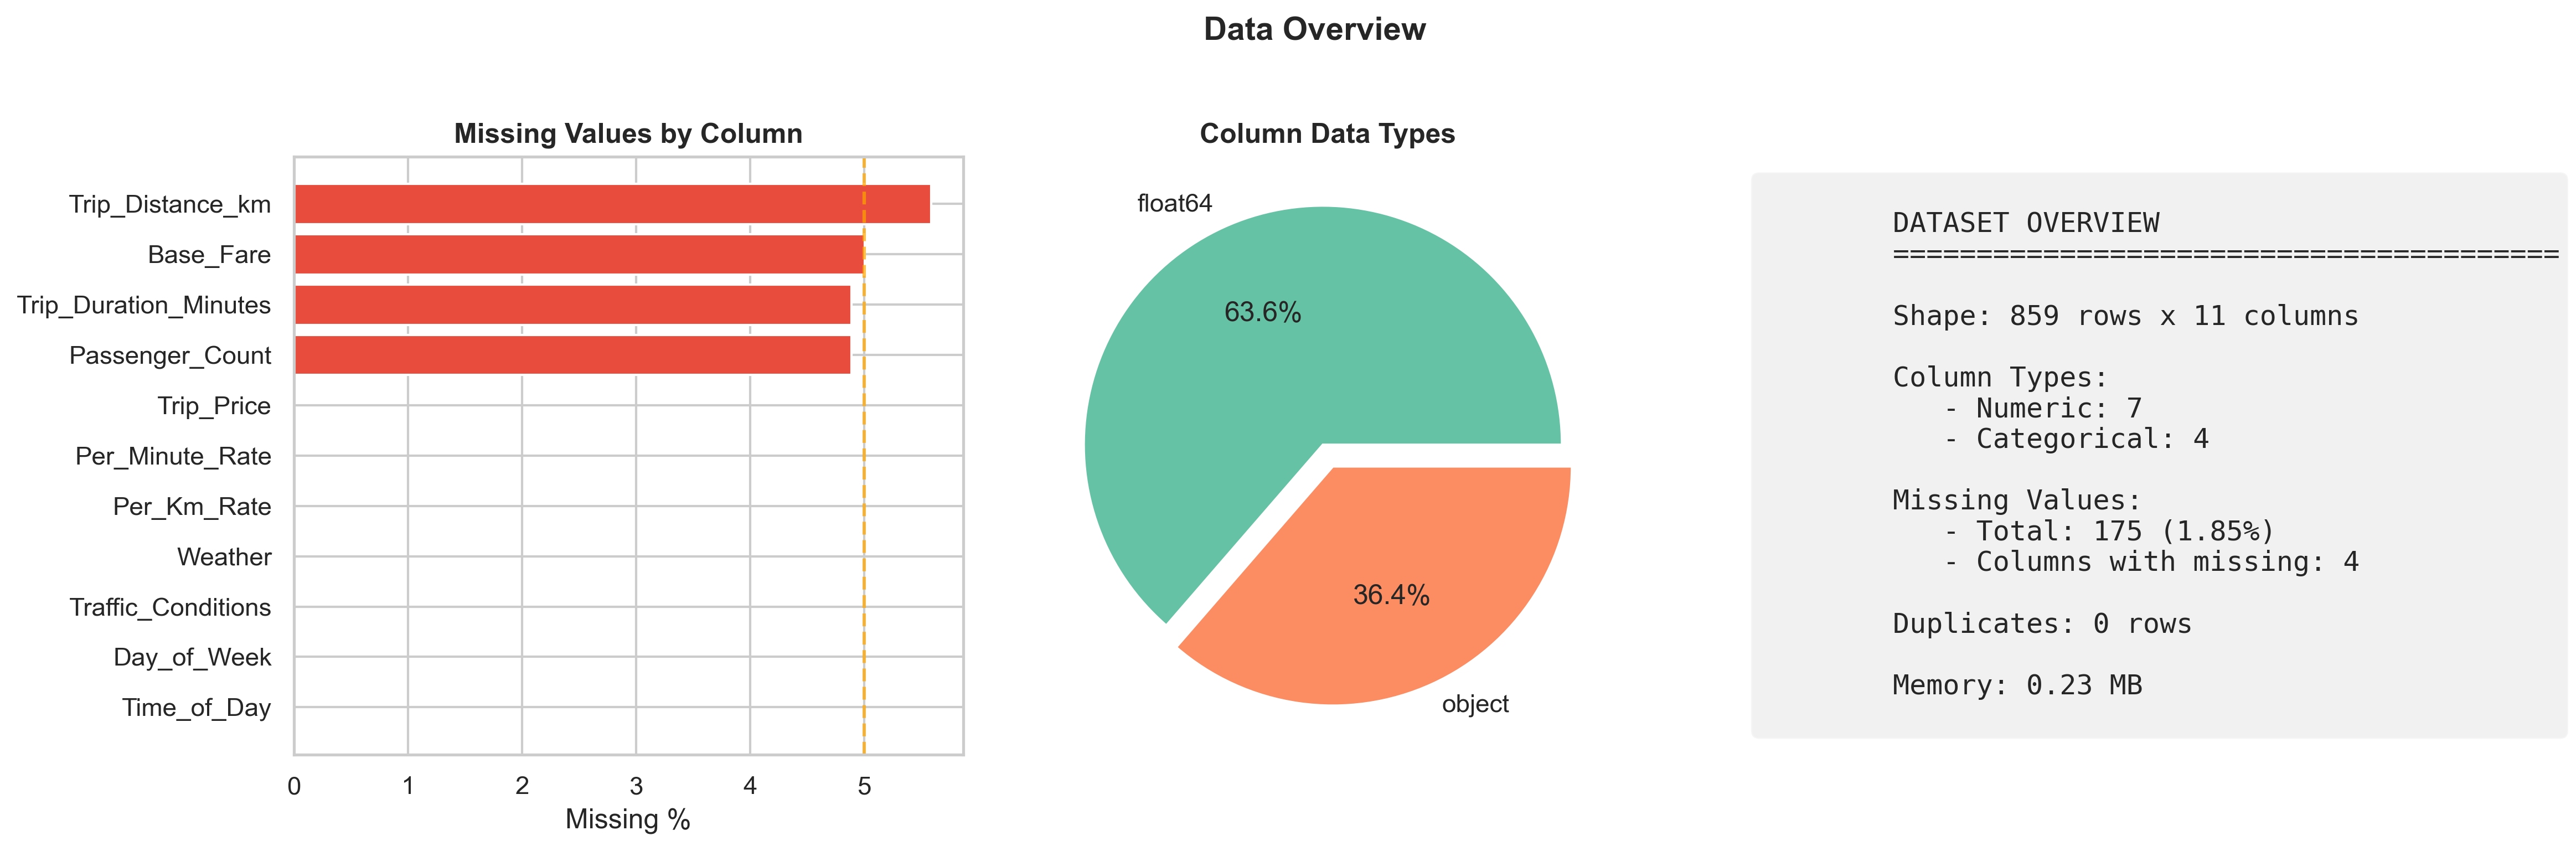
\includegraphics[width=0.95\textwidth]{../results/eda/01_data_overview.png}
\caption{Tổng quan dữ liệu: thông tin về shape, dtypes và missing values}
\label{fig:data_overview}
\end{figure}

\subsubsection{Phân phối các biến số}

\begin{figure}[H]
\centering
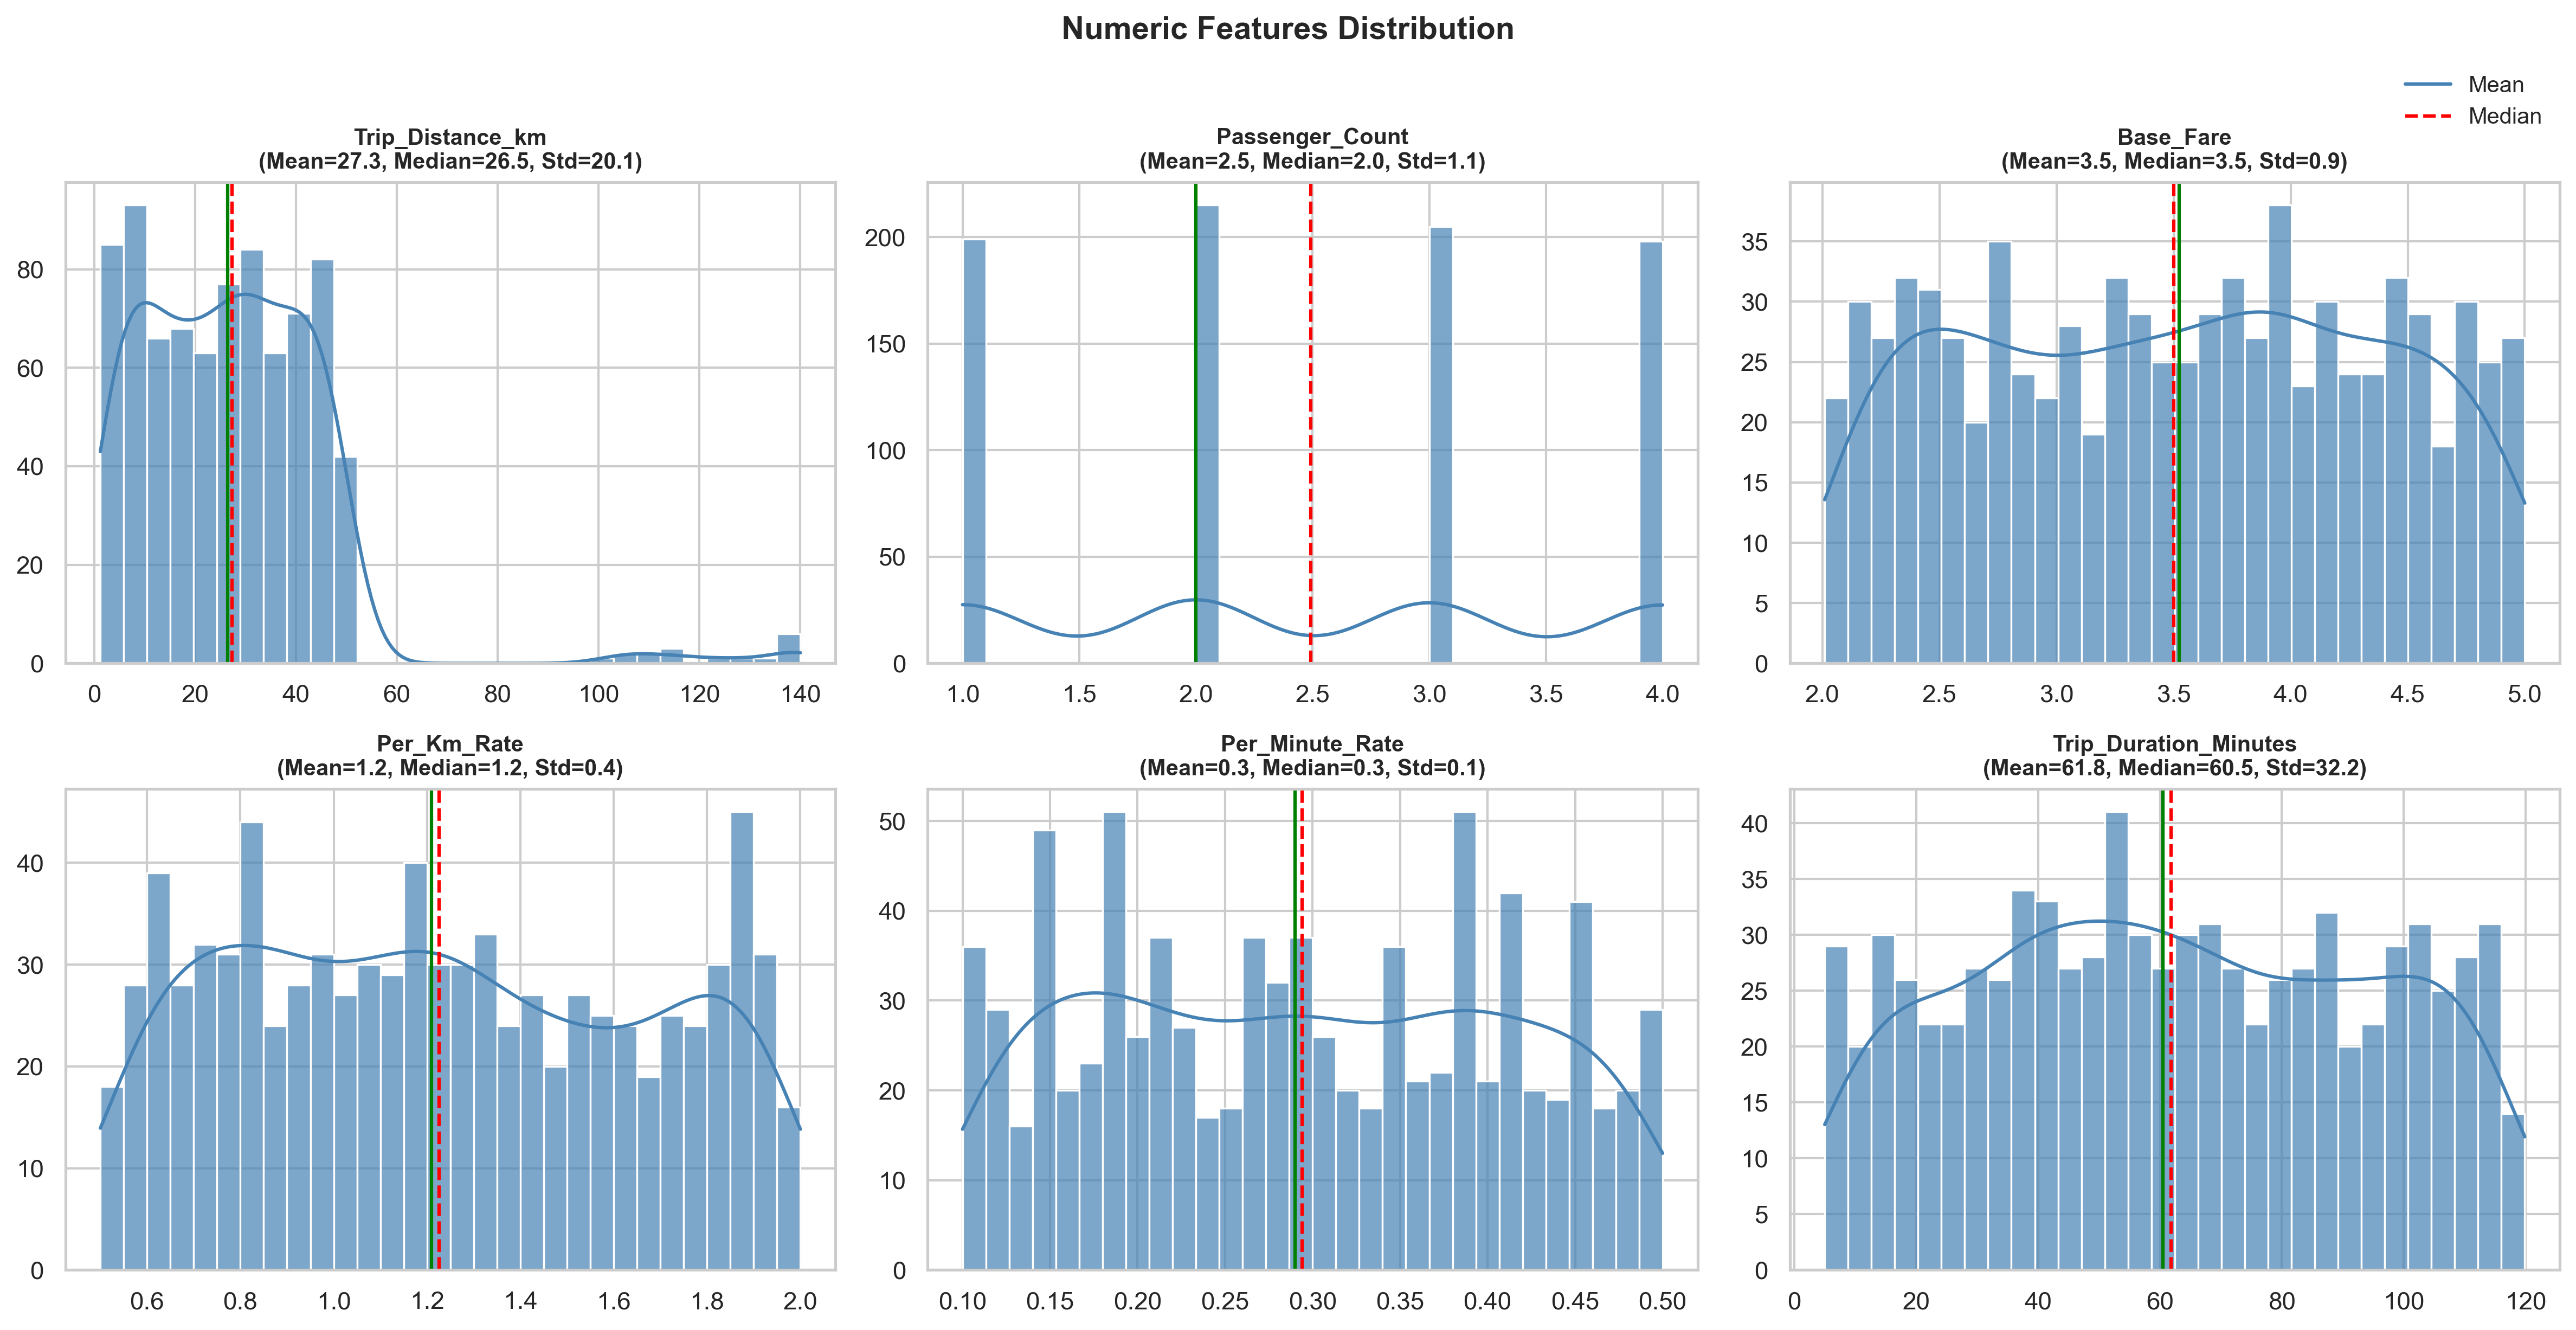
\includegraphics[width=0.95\textwidth]{../results/eda/02_numeric_distributions.png}
\caption{Phân phối của các biến số (numeric features) với histogram và KDE}
\label{fig:numeric_distributions}
\end{figure}

\subsubsection{Phân phối các biến phân loại}

\begin{figure}[H]
\centering
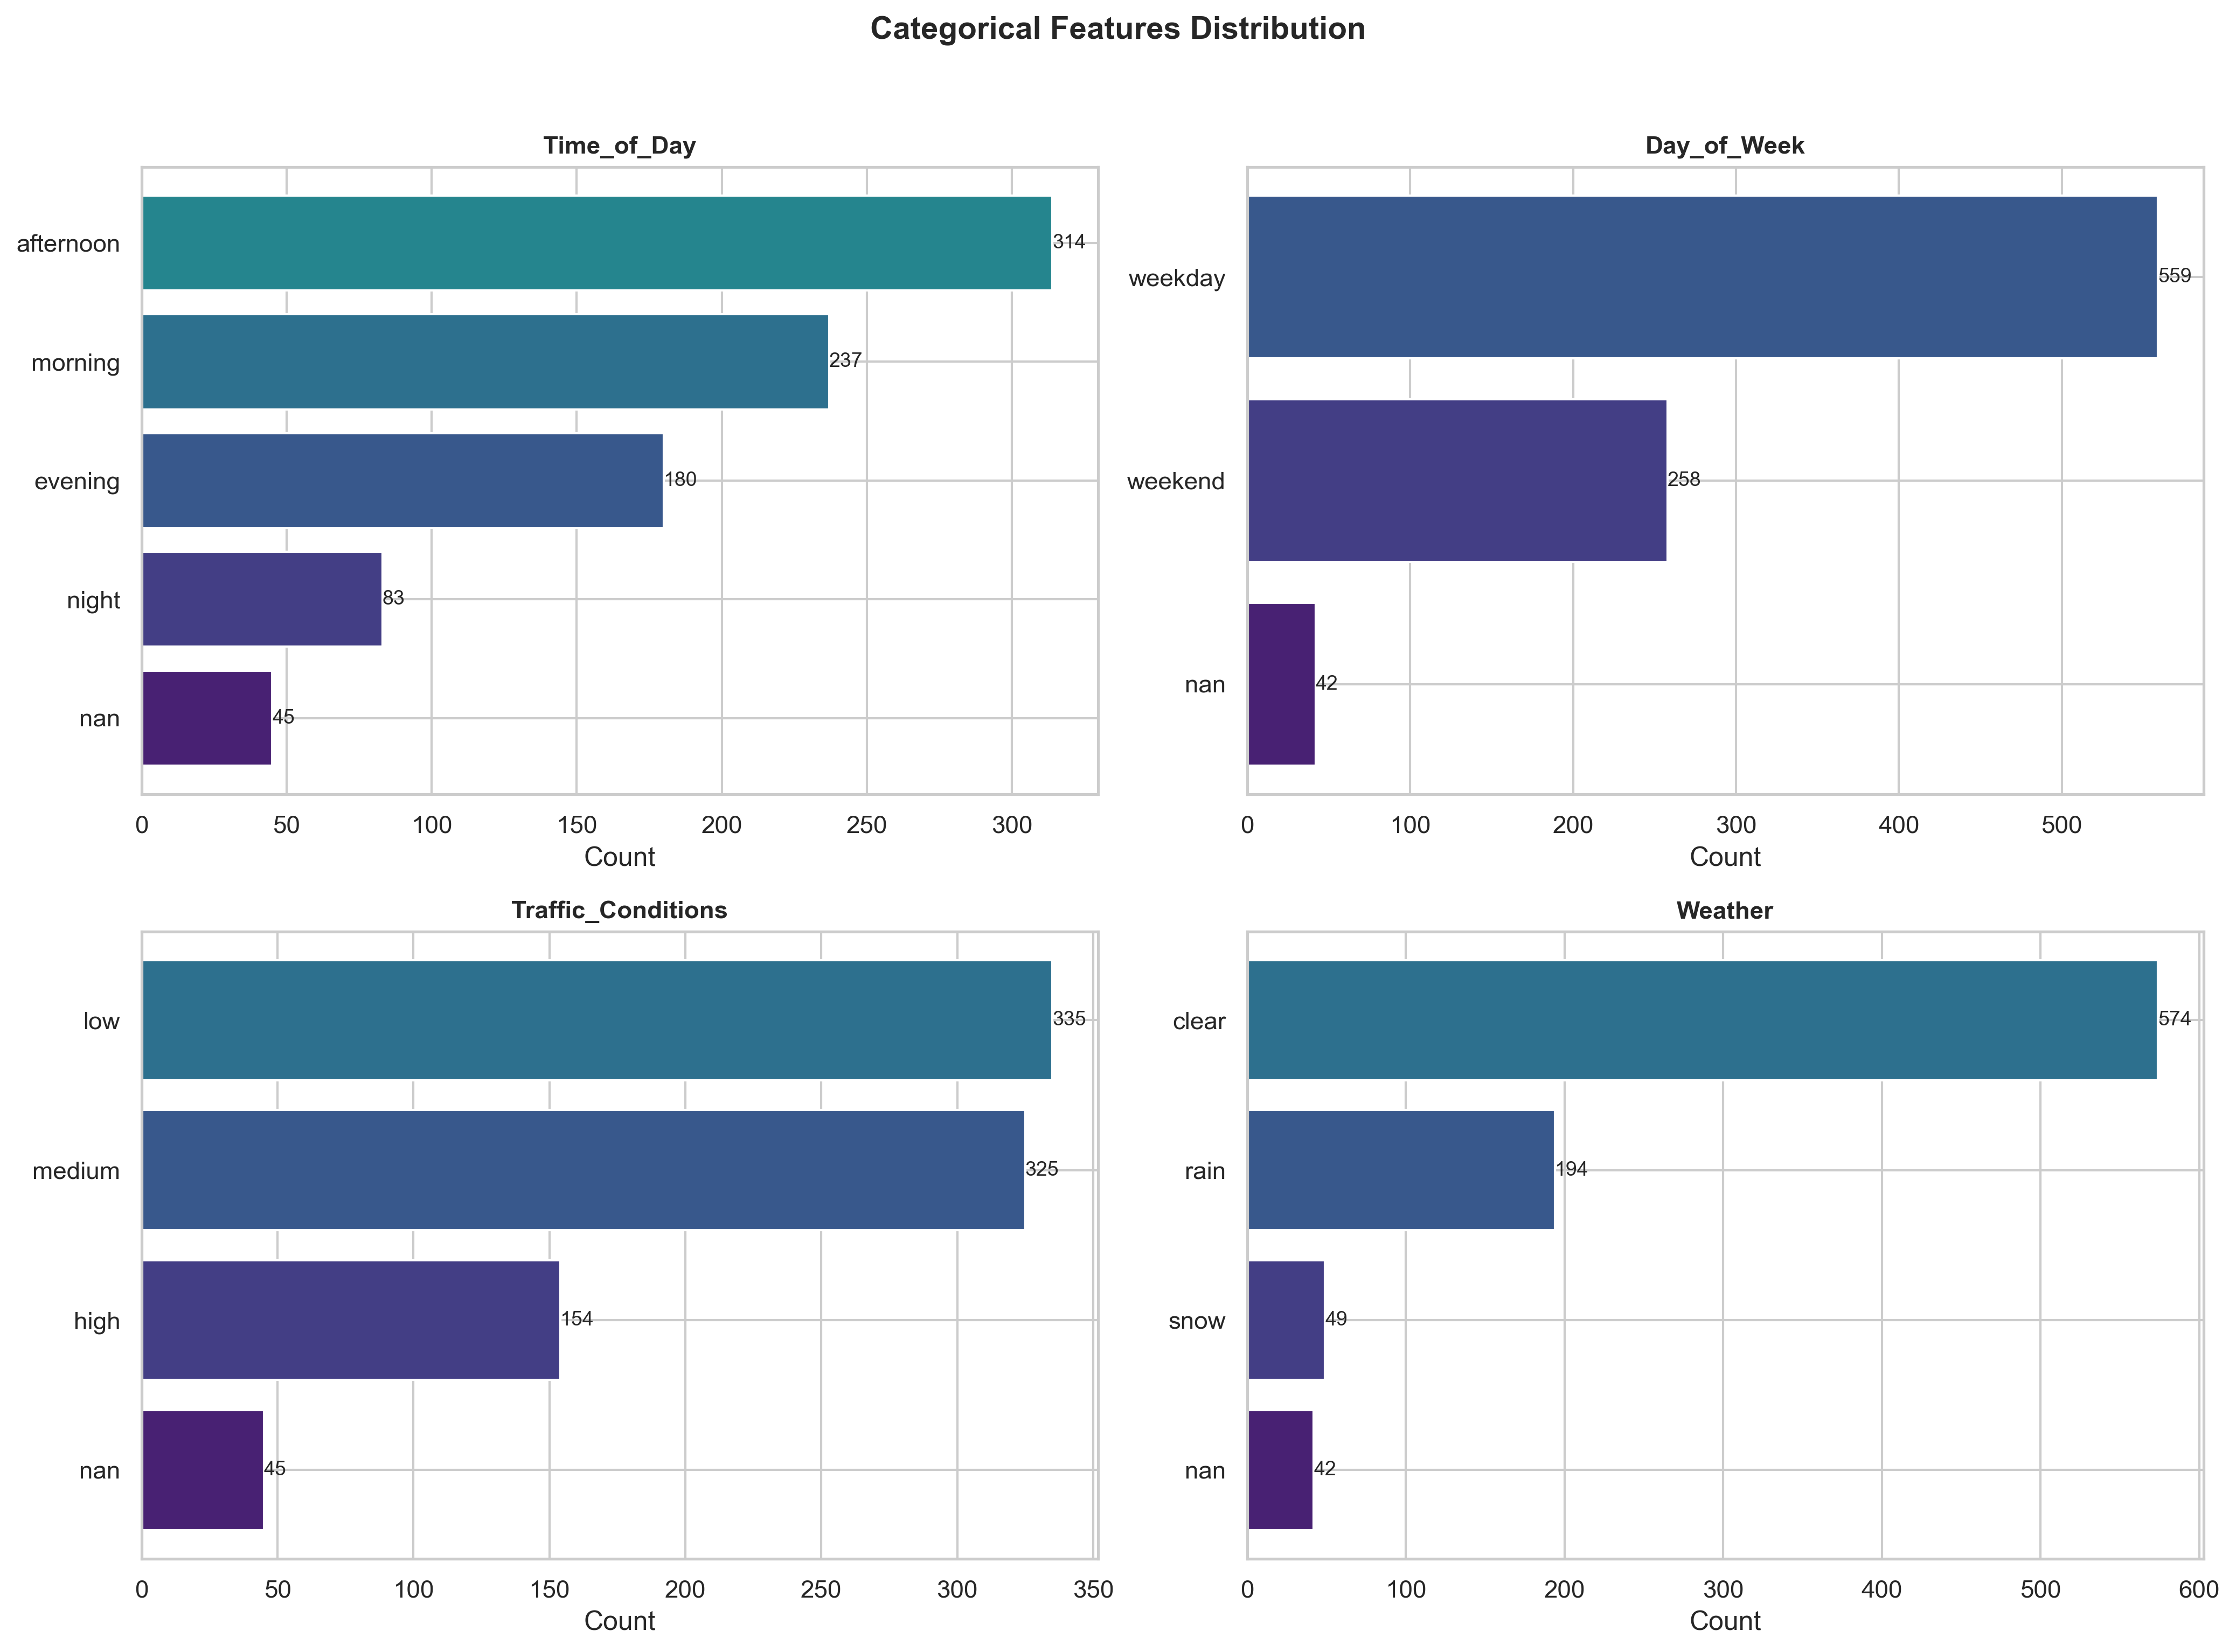
\includegraphics[width=0.95\textwidth]{../results/eda/03_categorical_distributions.png}
\caption{Phân phối của các biến phân loại (categorical features)}
\label{fig:categorical_distributions}
\end{figure}

\subsubsection{Ma trận tương quan}

\begin{figure}[H]
\centering
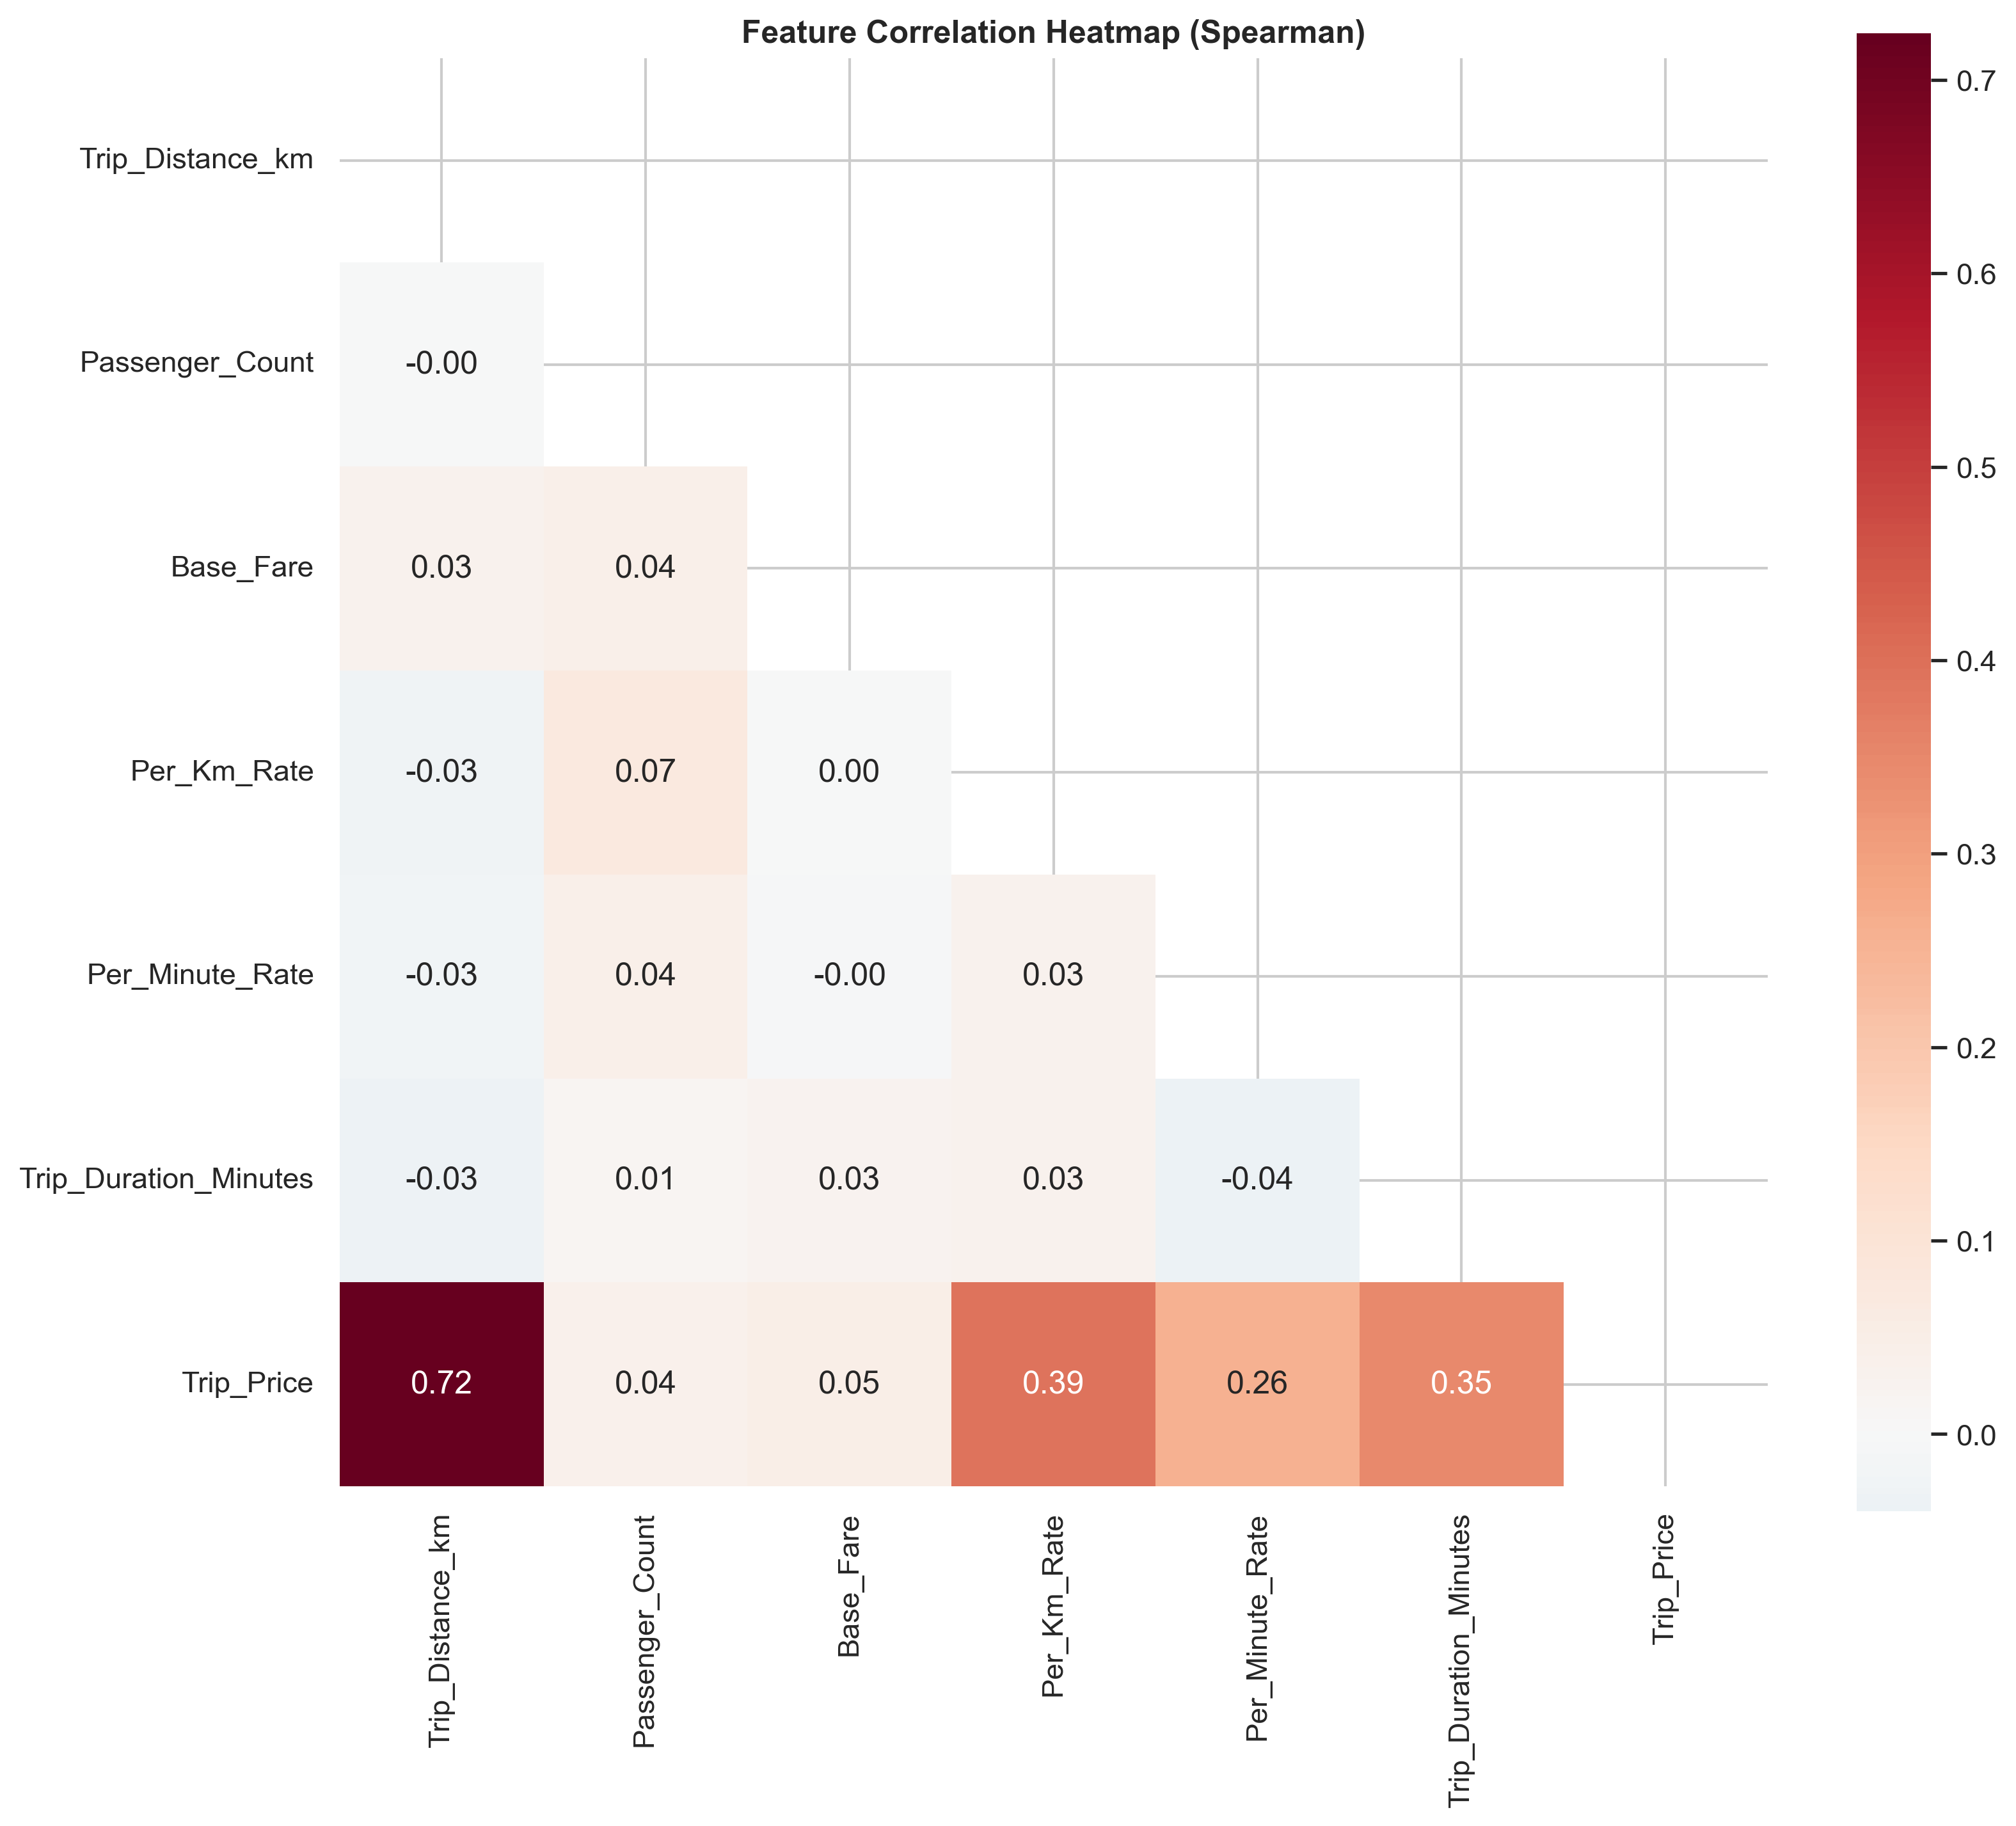
\includegraphics[width=0.85\textwidth]{../results/eda/04_correlation_heatmap.png}
\caption{Ma trận tương quan (Correlation Heatmap) giữa các biến số}
\label{fig:correlation_heatmap}
\end{figure}

\subsubsection{Phân tích biến mục tiêu}

\begin{figure}[H]
\centering
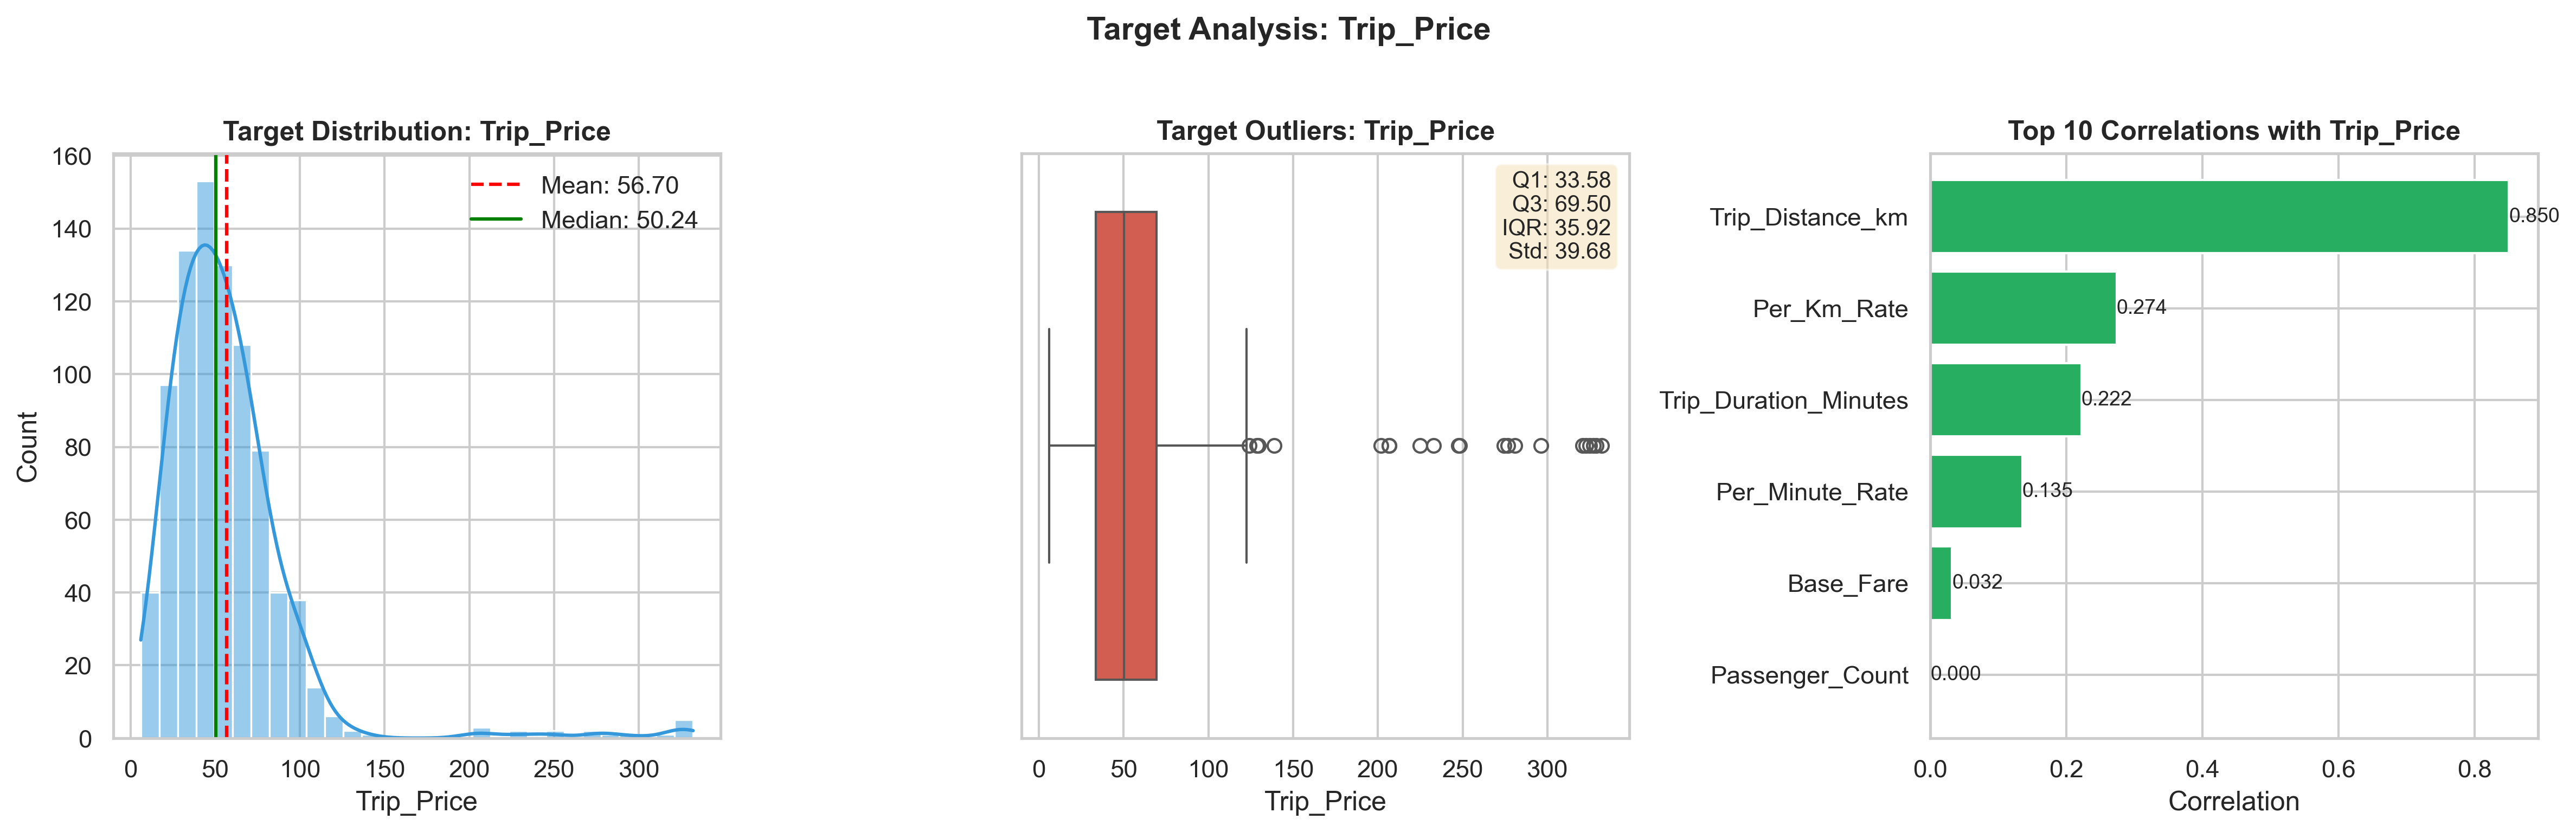
\includegraphics[width=0.95\textwidth]{../results/eda/05_target_analysis.png}
\caption{Phân tích chi tiết biến mục tiêu Trip\_Price}
\label{fig:target_analysis}
\end{figure}

\subsubsection{Phát hiện Outliers}

\begin{figure}[H]
\centering
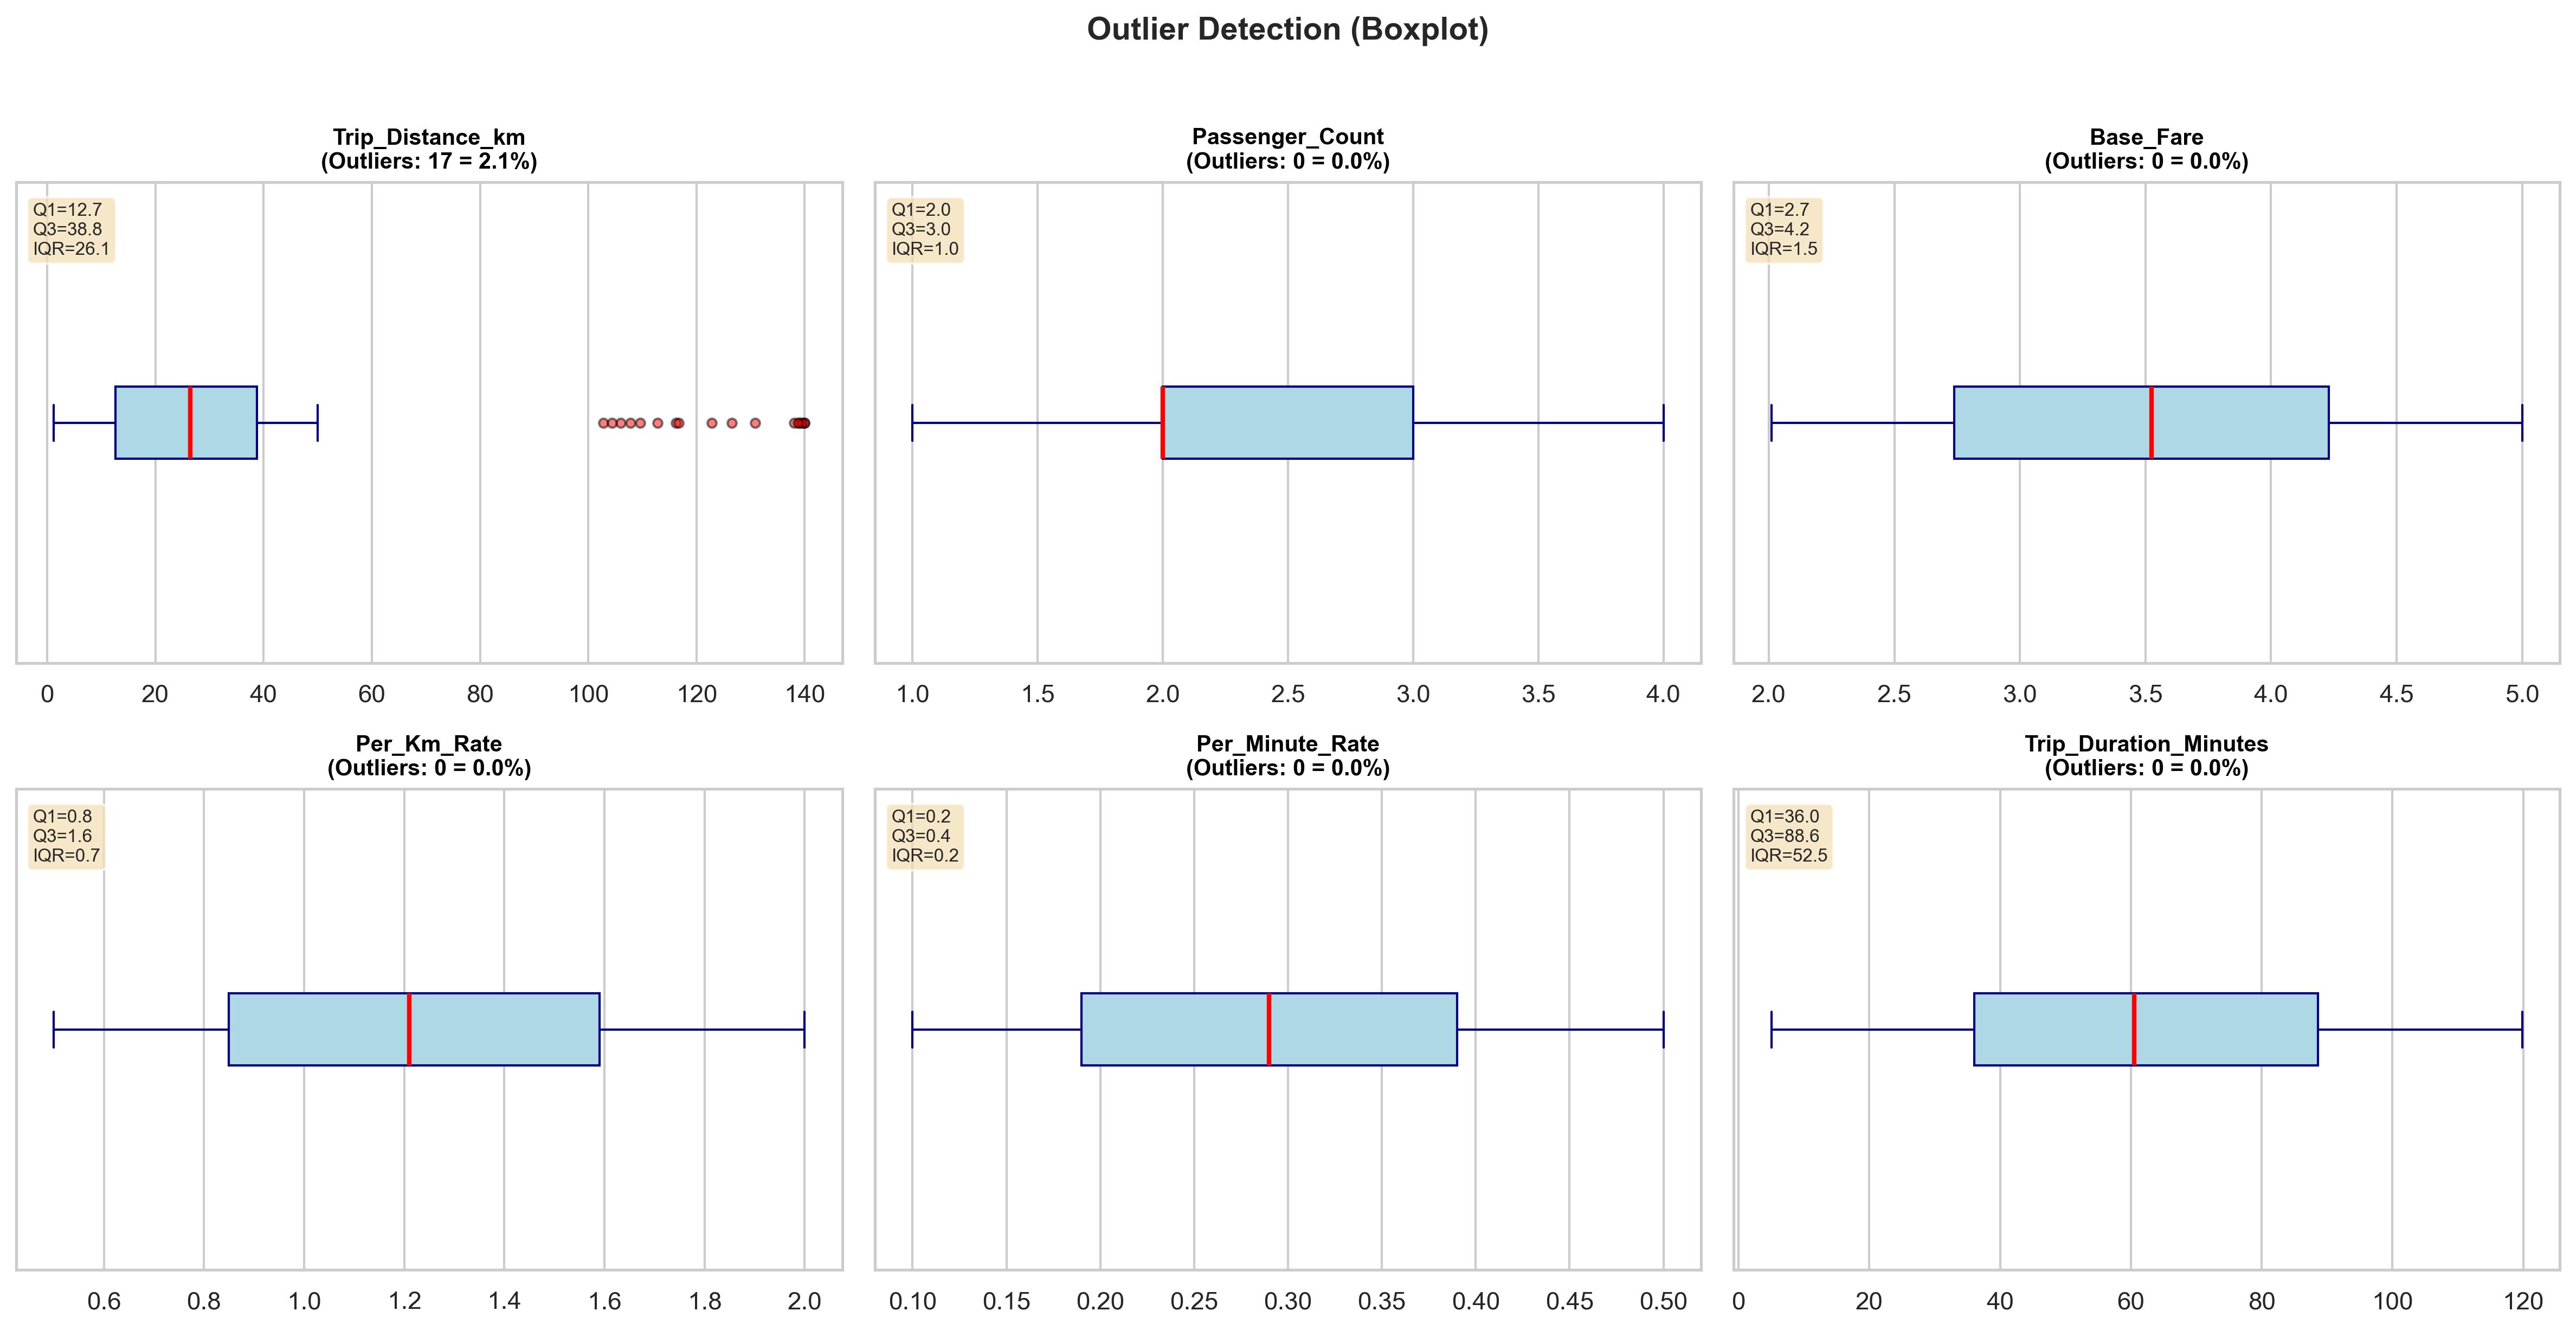
\includegraphics[width=0.95\textwidth]{../results/eda/06_outliers_boxplot.png}
\caption{Boxplot phát hiện outliers cho tất cả biến số}
\label{fig:outliers_boxplot}
\end{figure}

\subsection{Các biểu đồ Model Evaluation}

Dự án tạo ra 3 biểu đồ đánh giá mô hình trong thư mục \texttt{results/model/}:

\subsubsection{So sánh Metrics các mô hình}

\begin{figure}[H]
\centering
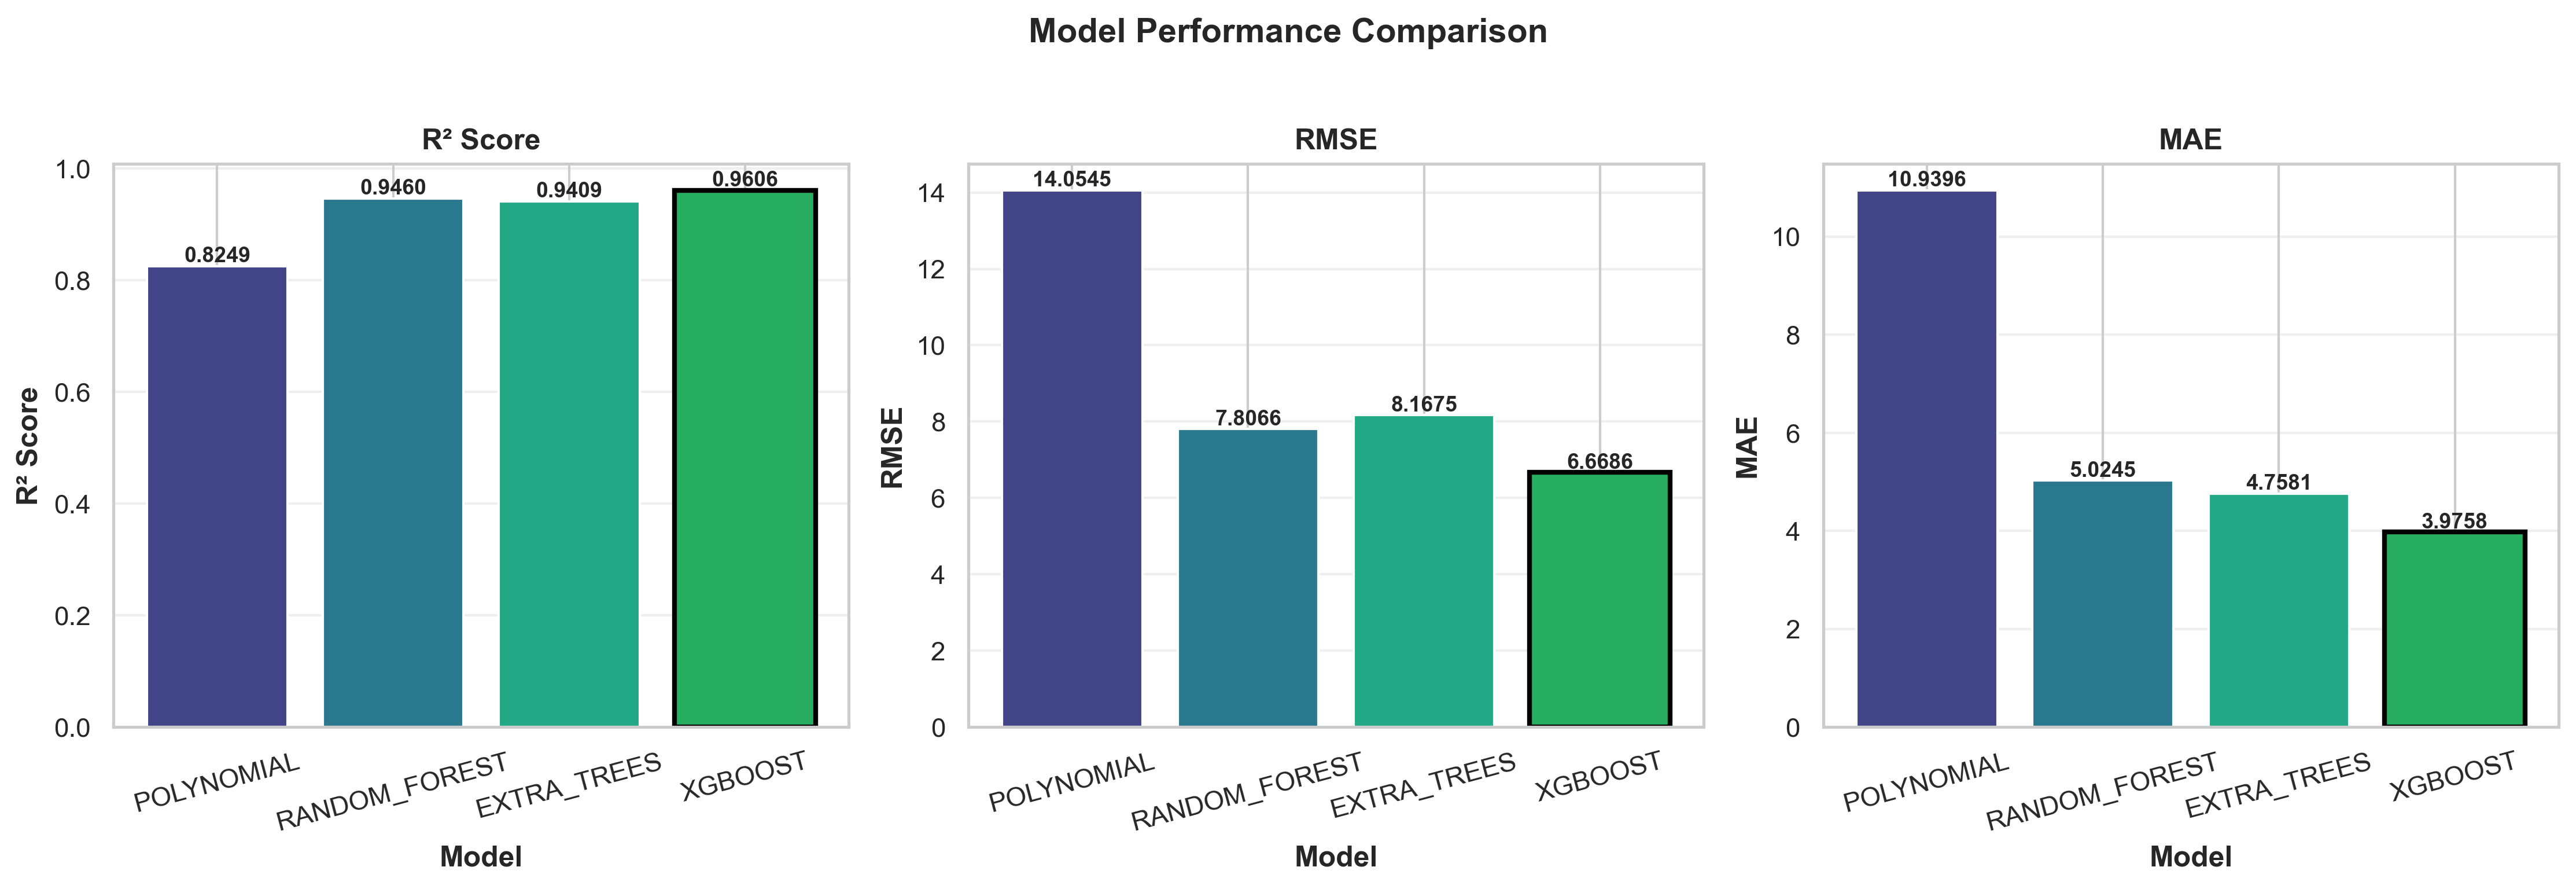
\includegraphics[width=0.95\textwidth]{../results/model/metrics_summary.png}
\caption{So sánh các metrics (RMSE, MAE, R²) của 4 mô hình}
\label{fig:metrics_summary}
\end{figure}

\subsubsection{Actual vs Predicted}

\begin{figure}[H]
\centering
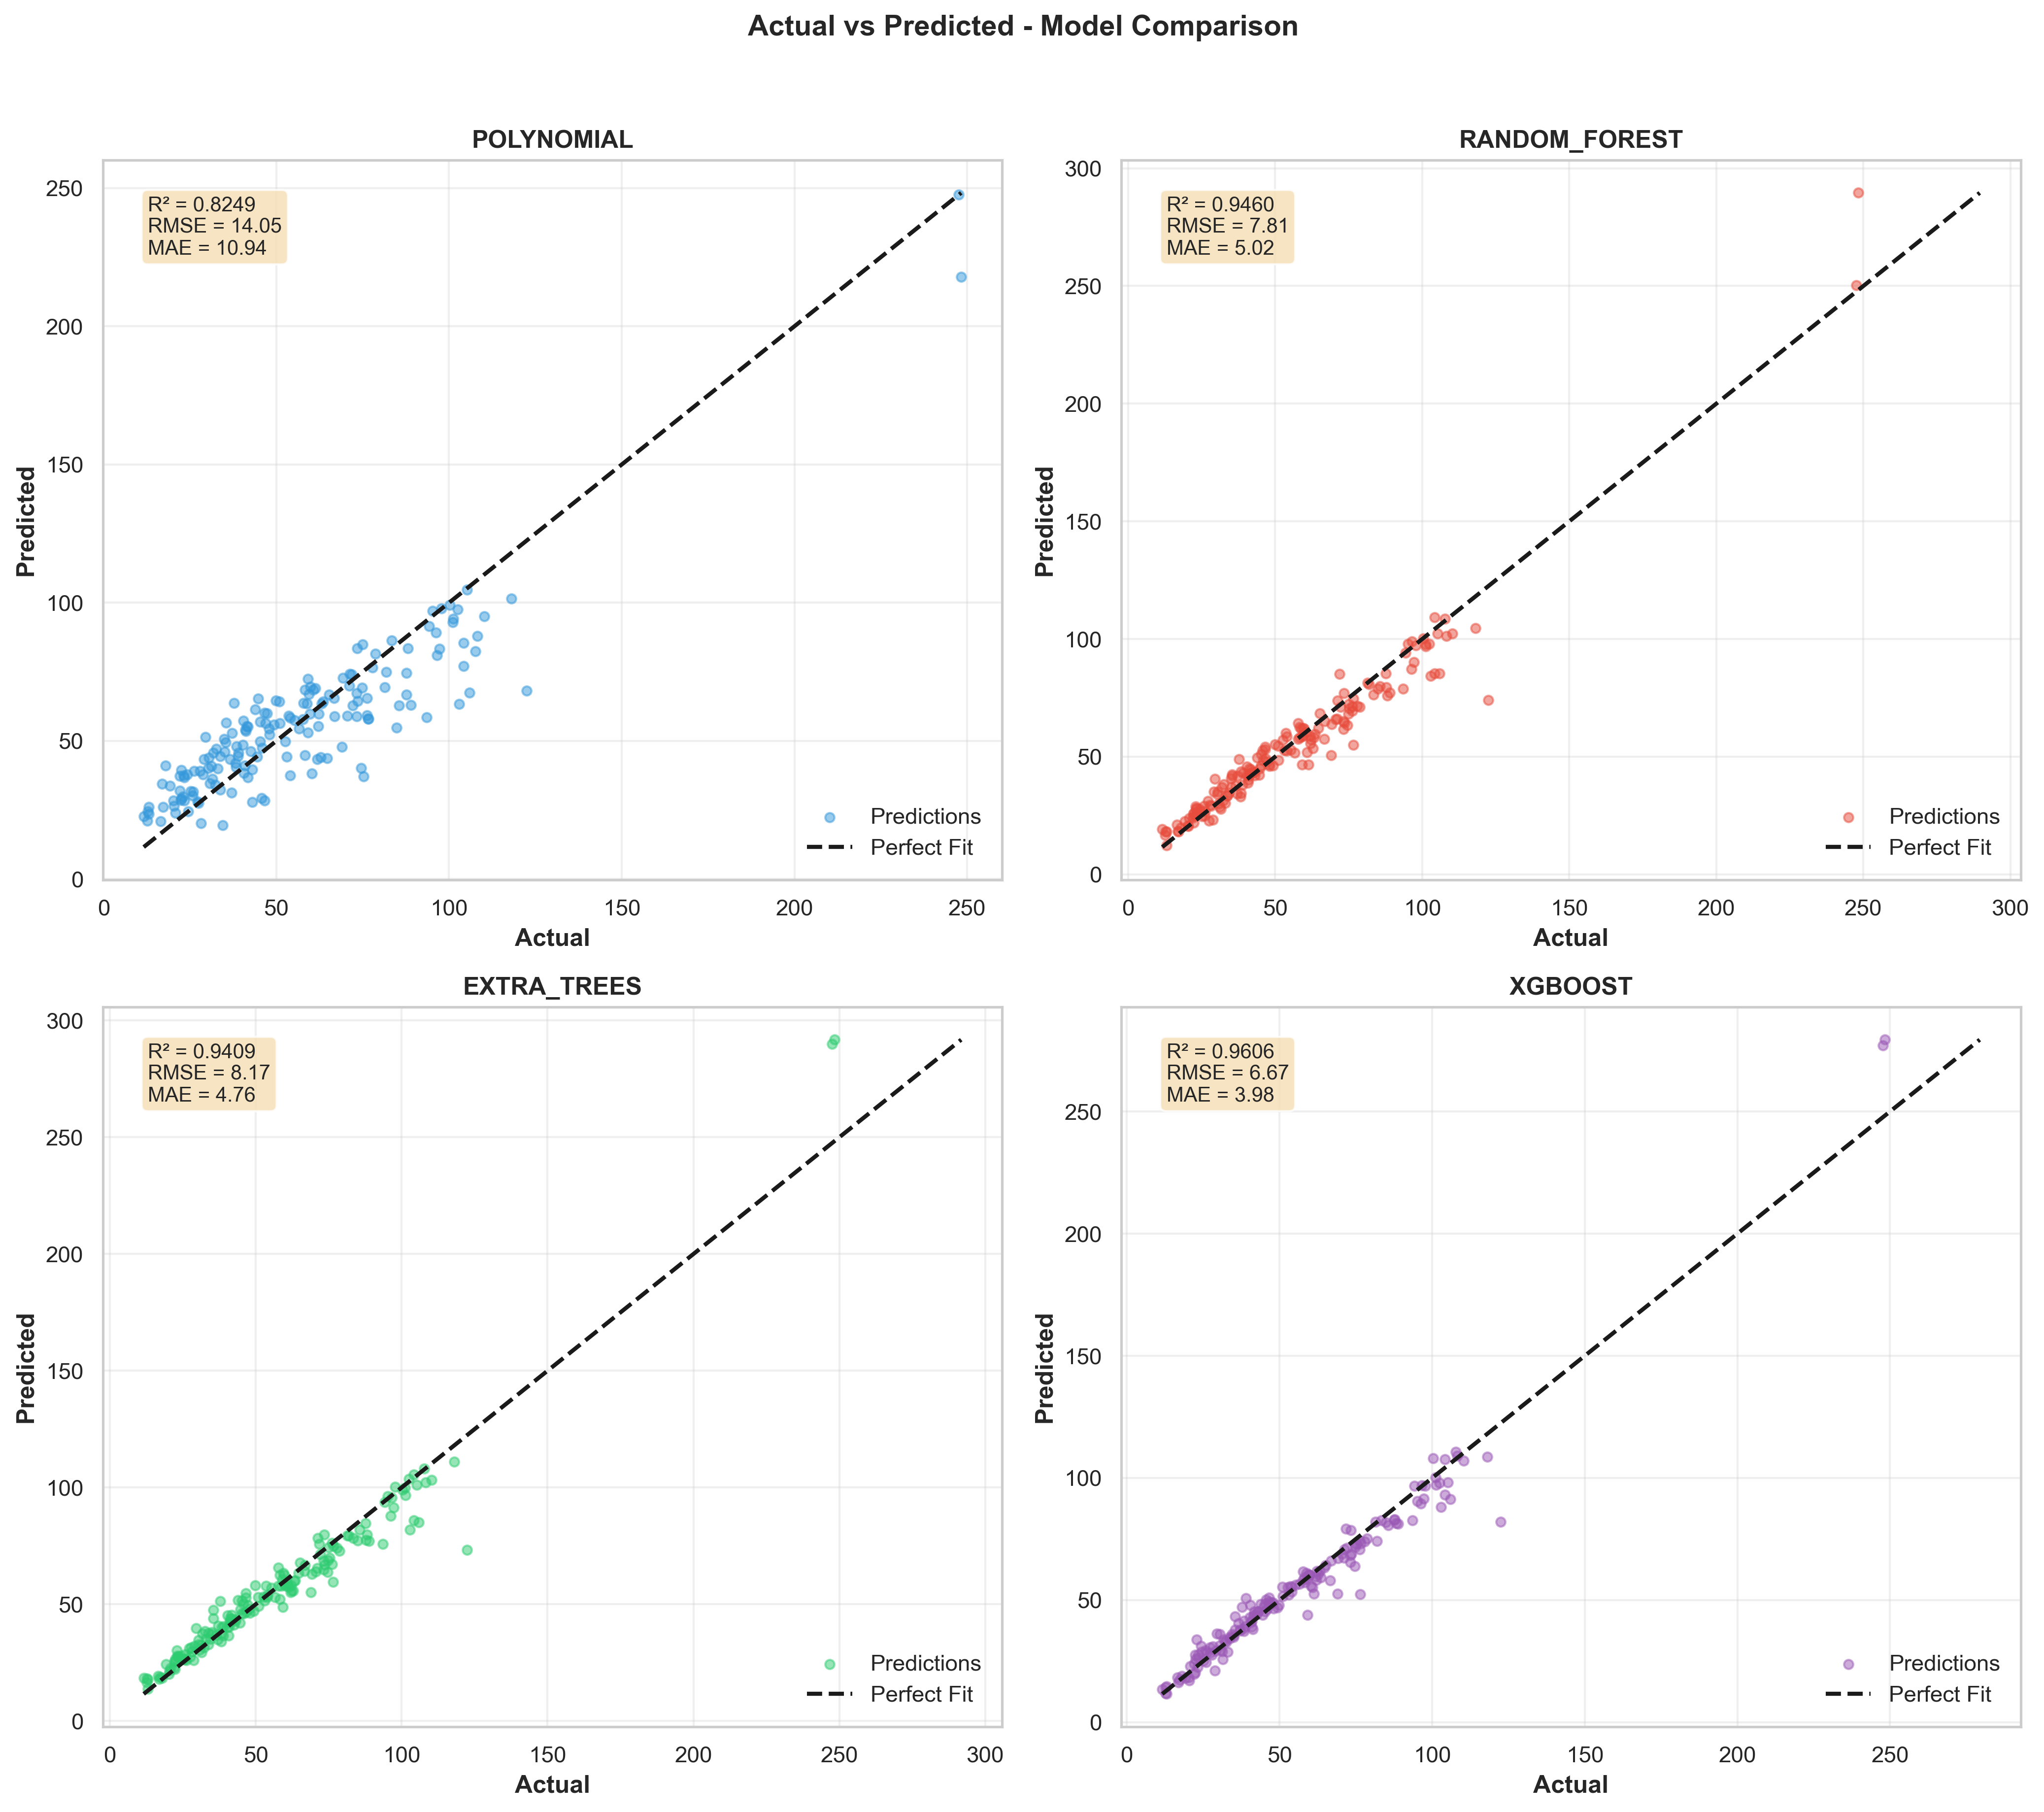
\includegraphics[width=0.95\textwidth]{../results/model/predictions_combined.png}
\caption{Scatter plot Actual vs Predicted cho 4 mô hình}
\label{fig:predictions_combined}
\end{figure}

\subsubsection{Feature Importance}

\begin{figure}[H]
\centering
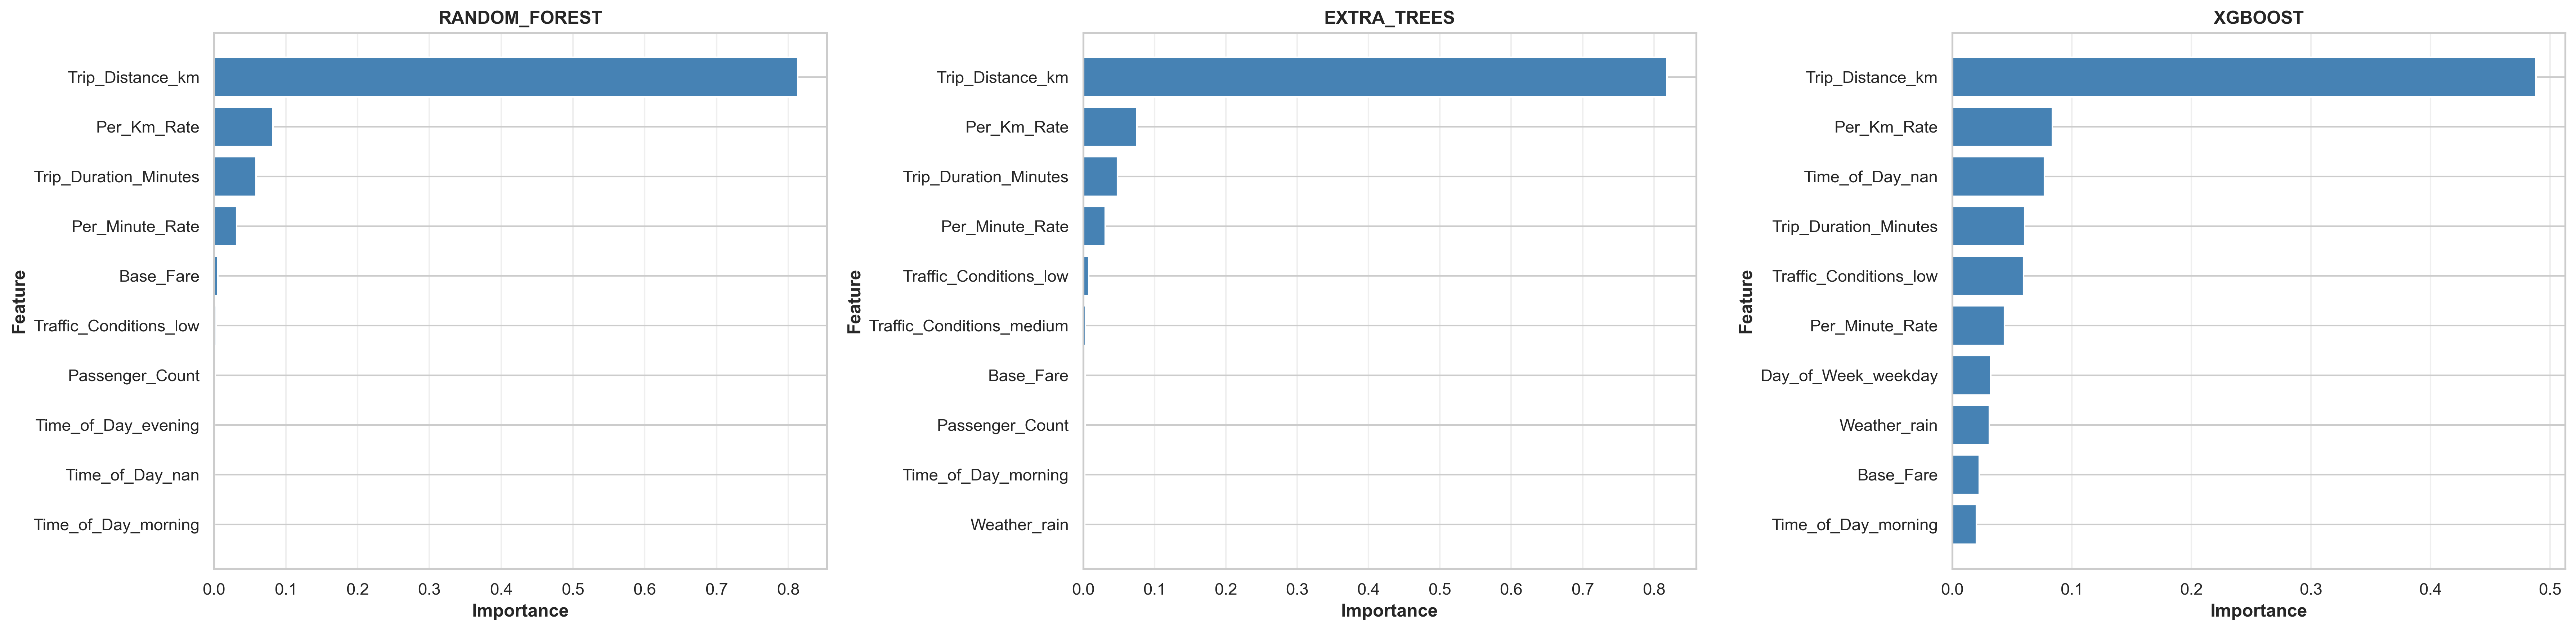
\includegraphics[width=0.95\textwidth]{../results/model/feature_importance_comparison.png}
\caption{So sánh Feature Importance của các tree-based models}
\label{fig:feature_importance}
\end{figure}

\subsection{Phân tích ý nghĩa các biểu đồ}

\subsubsection{Biểu đồ Correlation Heatmap (Hình \ref{fig:correlation_heatmap})}

\textbf{Mục đích:} Phát hiện mối tương quan giữa các biến

\textbf{Cách đọc:}
\begin{itemize}
    \item Giá trị gần 1: Tương quan dương mạnh
    \item Giá trị gần -1: Tương quan âm mạnh
    \item Giá trị gần 0: Không có tương quan tuyến tính
\end{itemize}

\textbf{Ứng dụng:}
\begin{itemize}
    \item Nhận diện features có correlation cao với target → features quan trọng
    \item Phát hiện multicollinearity (features tương quan cao với nhau) → có thể loại bỏ
\end{itemize}

\subsubsection{Biểu đồ Actual vs Predicted (Hình \ref{fig:predictions_combined})}

\textbf{Mục đích:} Đánh giá trực quan độ chính xác của mô hình

\textbf{Cách đọc:}
\begin{itemize}
    \item Điểm nằm trên đường y=x: Dự đoán chính xác
    \item Điểm phân tán quanh đường y=x: Mô hình tốt
    \item Điểm xa đường y=x: Sai số lớn
\end{itemize}

\subsubsection{Biểu đồ Feature Importance (Hình \ref{fig:feature_importance})}

\textbf{Mục đích:} Hiểu features nào ảnh hưởng nhiều nhất đến dự đoán

\textbf{Tính toán (cho tree-based models):}
\begin{itemize}
    \item Dựa trên tổng decrease in impurity (Gini/MSE) khi sử dụng feature để split
    \item Giá trị được chuẩn hóa để tổng = 1
\end{itemize}

\textbf{Ứng dụng:}
\begin{itemize}
    \item Feature selection: Giữ lại features quan trọng
    \item Model interpretation: Giải thích mô hình cho stakeholders
    \item Domain insight: Hiểu yếu tố nào ảnh hưởng giá cước taxi
\end{itemize}

% =====================================
% CHƯƠNG 9: HƯỚNG DẪN SỬ DỤNG
% =====================================
\section{Hướng dẫn sử dụng}

\subsection{Yêu cầu hệ thống}

\begin{itemize}
    \item \textbf{Python:} Phiên bản 3.8 trở lên
    \item \textbf{RAM:} Tối thiểu 4GB (khuyến nghị 8GB khi chạy optimization)
    \item \textbf{Hệ điều hành:} Windows, Linux, hoặc macOS
\end{itemize}

\subsection{Cài đặt môi trường}

\textbf{Bước 1:} Clone hoặc download project về máy

\textbf{Bước 2:} Cài đặt các thư viện cần thiết thông qua pip:
\begin{verbatim}
pip install -r requirements.txt
\end{verbatim}

\textbf{Bước 3:} Kiểm tra cài đặt thành công bằng cách import các thư viện chính

\subsection{Chạy Pipeline}

\subsubsection{Chạy toàn bộ pipeline}

Sử dụng file \texttt{main.py} với các tùy chọn:

\begin{table}[H]
\centering
\caption{Các tùy chọn command line}
\begin{tabular}{|l|p{8cm}|}
\hline
\textbf{Tùy chọn} & \textbf{Mô tả} \\
\hline
(không có) & Chạy với hyperparameters mặc định (nhanh, ~2 giây) \\
\hline
\texttt{--optimize} & Chạy Optuna optimization cho hyperparameters (chậm hơn, kết quả tốt hơn) \\
\hline
\texttt{--no-viz} & Bỏ qua việc vẽ biểu đồ \\
\hline
\texttt{--skip-download} & Bỏ qua download dữ liệu nếu đã có \\
\hline
\end{tabular}
\end{table}

\subsubsection{Dự đoán với model đã train}

Sử dụng file \texttt{predict.py}:

\begin{table}[H]
\centering
\caption{Các tùy chọn predict.py}
\begin{tabular}{|l|p{8cm}|}
\hline
\textbf{Tùy chọn} & \textbf{Mô tả} \\
\hline
\texttt{--input <file>} & Đường dẫn đến file CSV cần dự đoán \\
\hline
\texttt{--output <file>} & Đường dẫn file output (mặc định: predictions.csv) \\
\hline
\texttt{--model <name>} & Chọn model cụ thể (polynomial, random\_forest, extra\_trees, xgboost) \\
\hline
\texttt{--interactive} & Chế độ nhập từng giá trị thủ công \\
\hline
\end{tabular}
\end{table}

\subsection{Quy trình sử dụng Module}

\subsubsection{Phase 1: Load và Clean dữ liệu}

Sử dụng \texttt{DataLoader} để đọc và làm sạch dữ liệu ban đầu:
\begin{enumerate}
    \item Tạo instance từ file dữ liệu
    \item Xóa duplicates
    \item Chuẩn hóa giá trị text
    \item Áp dụng constraints
    \item Lấy DataFrame đã xử lý
\end{enumerate}

\subsubsection{Phase 2: Chia Train/Test}

Sử dụng \texttt{train\_test\_split} từ scikit-learn với tỉ lệ 80/20 và random\_state cố định để đảm bảo reproducibility.

\subsubsection{Phase 3: Transform dữ liệu}

Sử dụng \texttt{DataTransformer}:
\begin{enumerate}
    \item Khởi tạo với train data
    \item Gọi \texttt{fit\_transform()} trên train
    \item Gọi \texttt{transform\_new\_data()} trên test
    \item Lưu state để dùng cho inference sau này
\end{enumerate}

\subsubsection{Phase 4: Training và Evaluation}

Sử dụng \texttt{ModelTrainer}:
\begin{enumerate}
    \item Khởi tạo với X\_train, X\_test, y\_train, y\_test
    \item Gọi \texttt{train\_all()} để train tất cả models
    \item Gọi \texttt{compare\_models()} để so sánh và chọn best model
    \item Lưu models và kết quả
\end{enumerate}

% =====================================
% CHƯƠNG 10: KẾT LUẬN
% =====================================
\section{Kết luận}

\subsection{Tổng kết}

Dự án đã hoàn thành các mục tiêu đề ra:

\begin{enumerate}
    \item \textbf{Pipeline hoàn chỉnh}: Xây dựng thành công pipeline từ tiền xử lý đến dự đoán với kiến trúc module hóa, dễ bảo trì.
    
    \item \textbf{Lập trình OOP}: Áp dụng các kỹ thuật Python nâng cao như:
    \begin{itemize}
        \item Abstract Base Class
        \item Property, staticmethod, classmethod
        \item Type hints và docstrings
        \item Exception handling
        \item Logging
    \end{itemize}
    
    \item \textbf{So sánh mô hình}: Huấn luyện và đánh giá 4 mô hình, với \textbf{Extra Trees} đạt hiệu suất tốt nhất (R² = 0.953).
    
    \item \textbf{Tối ưu hyperparameters}: Tích hợp Optuna để tự động tìm kiếm hyperparameters tối ưu.
    
    \item \textbf{Trực quan hóa}: Tạo các biểu đồ EDA và đánh giá model chuyên nghiệp.
\end{enumerate}

\subsection{Hạn chế}

\begin{itemize}
    \item Chưa thử nghiệm với các mô hình Deep Learning
    \item Chưa có feature engineering phức tạp hơn (interaction features, domain-specific features)
    \item Cần tối ưu XGBoost để đạt hiệu suất tốt hơn
\end{itemize}

\subsection{Hướng phát triển}

\begin{itemize}
    \item Thử nghiệm thêm các mô hình như LightGBM, CatBoost, Neural Networks
    \item Áp dụng SHAP để giải thích model
    \item Xây dựng API để deploy model
    \item Tích hợp MLflow để quản lý experiments
\end{itemize}

% =====================================
% TÀI LIỆU THAM KHẢO
% =====================================
\section*{Tài liệu tham khảo}
\addcontentsline{toc}{section}{Tài liệu tham khảo}

\begin{enumerate}
    \item Pedregosa, F., et al. (2011). Scikit-learn: Machine Learning in Python. JMLR 12, pp. 2825-2830.
    
    \item Chen, T., \& Guestrin, C. (2016). XGBoost: A Scalable Tree Boosting System. KDD'16.
    
    \item Akiba, T., et al. (2019). Optuna: A Next-generation Hyperparameter Optimization Framework. KDD'19.
    
    \item Geurts, P., Ernst, D., \& Wehenkel, L. (2006). Extremely randomized trees. Machine Learning, 63(1), 3-42.
    
    \item McKinney, W. (2010). Data Structures for Statistical Computing in Python. Proceedings of the 9th Python in Science Conference.
\end{enumerate}

% =====================================
% PHỤ LỤC
% =====================================
\appendix
\section{Phụ lục: Danh sách thư viện sử dụng}

\begin{table}[H]
\centering
\caption{Requirements.txt}
\label{tab:requirements}
\begin{tabular}{|l|l|p{6cm}|}
\hline
\textbf{Thư viện} & \textbf{Version} & \textbf{Mục đích} \\
\hline
pandas & $\geq$ 1.3.0 & Xử lý dữ liệu \\
\hline
numpy & $\geq$ 1.21.0 & Tính toán số học \\
\hline
scikit-learn & $\geq$ 1.0.0 & Machine Learning \\
\hline
xgboost & $\geq$ 1.5.0 & XGBoost algorithm \\
\hline
optuna & $\geq$ 3.0.0 & Hyperparameter optimization \\
\hline
matplotlib & $\geq$ 3.4.0 & Visualization \\
\hline
seaborn & $\geq$ 0.11.0 & Statistical visualization \\
\hline
joblib & $\geq$ 1.1.0 & Model serialization \\
\hline
\end{tabular}
\end{table}

\section{Phụ lục: Phân công công việc}

\begin{table}[H]
\centering
\caption{Phân công công việc trong nhóm}
\label{tab:task_assignment}
\begin{tabular}{|c|l|p{6cm}|}
\hline
\textbf{STT} & \textbf{Thành viên} & \textbf{Công việc} \\
\hline
1 & [Họ tên SV 1] & [Mô tả công việc] \\
\hline
2 & [Họ tên SV 2] & [Mô tả công việc] \\
\hline
3 & [Họ tên SV 3] & [Mô tả công việc] \\
\hline
\end{tabular}
\end{table}

\end{document}
